% % part: 微分方程
% % chap: 倒向随机微分方程(Backward Stochastic Dierential Equations)


% \documentclass[UTF8]{ctexbook}

% \ctexset{
%     part/number = \chinese{part}
% }
% \usepackage{multirow}
% \usepackage{amsmath}% ams 数学公式
% \usepackage{amsfonts}% ams 数学字体
% \usepackage{bbm}%重影字体
% \usepackage{amssymb,latexsym}% ams 数学符号与LaTeX数学符号
% \usepackage{mathrsfs}% 花式符号
% \usepackage{ntheorem}%定理、定义、证明
%     \theoremstyle{nonumberplain}
%     \theoremheaderfont{\bfseries}
%     \theorembodyfont{\normalfont}
%     \theoremsymbol{$\square$}
%     \newtheorem{Proof}{\hskip 2em 证明}
%     \newtheorem{theorem}{\hspace{2em}定理}[chapter]
%     \newtheorem{definition}{\hspace{2em}定义}[chapter] % 如果没有章, 只有节, 把上面的[chapter]改成[section]
%     \newtheorem{axiom}[definition]{\hspace{2em}公理}
%     \newtheorem{lemma}[definition]{\hspace{2em}引理}
%     \newtheorem{proposition}[definition]{\hspace{2em}命题}
%     \newtheorem{corollary}[definition]{\hspace{2em}推论}
%     \newtheorem{remark}{\hspace{2em}注}[chapter] %类似地定义其他“题头”. 这里“注”的编号与定义、定理等是分开的
%     \newtheorem{Assumption}{\hspace{2em}假设}[chapter]

% %算法伪代码
% %http://blog.csdn.net/lwb102063/article/details/53046265
% \usepackage{algorithm}
% \usepackage{algorithmicx}
% \usepackage{algpseudocode}
%     \floatname{algorithm}{算法}
%     \renewcommand{\algorithmicrequire}{\textbf{输入:}}
%     \renewcommand{\algorithmicensure}{\textbf{输出:}}
% % 罗马数字:示例:\rom{2}
% \makeatletter
% \newcommand*{\rom}[1]{\expandafter\@slowromancap\romannumeral #1@}
% \makeatother

% \usepackage{enumerate}%itemiz环境。\begin{enumerate}[step 1][a)]可以使用 A,a,I,i,1 作为可选项产生 \Alph,\alph,\Roman,\roman,\arabic 的效果
% \usepackage{cite}%参考文献
%     \bibliographystyle{plain}
% \usepackage{extarrows}% 带参数的箭头
% \usepackage{hyperref}% 超链接
% \usepackage{pifont}%然后在正文输入\ding{172}~\ding{211}得到相应数字,要是要①就输入:\ding{172}②就输:\ding{173}
% %\usepackage[CJKbookmarks, colorlinks, bookmarksnumbered=true,pdfstartview=FitH,linkcolor=black,citecolor=black]{hyperref}%超链接的格式设置
% \hypersetup{
%     colorlinks=false,% 去掉超链接颜色
%     pdfborder=0 0 0% 取消超链接的边框
% }
% \usepackage{graphicx}% 图片管理
% \usepackage{caption}
% \usepackage{subcaption}%并排的图各有标题
% \graphicspath{{images/}}% 设置图片搜索路径
% \usepackage{float,varwidth}% 浮动体
% \usepackage{booktabs}% 三线表
% \usepackage{fancyhdr}% 页眉设置
% \usepackage{xcolor}% 颜色宏包
% \usepackage{colortbl}% 彩色表格
% \usepackage{listings}% 代码高亮
% \usepackage{caption}% 对标题进行控制,如让\caption标题的字体缩小一号,同时数字标签使用粗体可以用:\usepackage[font=small,labelfont=bf]{caption}
% \usepackage{xfrac,upgreek}%分别是行间公式如a/b的形式(将原来的命令\frac改成\sfrac)和希腊字体的宏包的
% \usepackage{mathtools}%lgathered和rgathered环境把公式向左向右对齐
% \usepackage{tabularx}%提供自动延伸的表列,(X列格式说明符),文字过长时可以自动转行
% \usepackage{longtable}%长表格
% \usepackage{enumitem}%enumerate宏包的升级
% \usepackage{harpoon}%数学公式的矢量
% \usepackage{bookmark}%目录的书签
% \renewcommand{\headwidth}{\textwidth}%图片并排,这个要列在所有宏包的后面
% \definecolor{codegreen}{rgb}{0,0.6,0}
% \definecolor{codegray}{rgb}{0.5,0.5,0.5}
% \definecolor{codepurple}{rgb}{0.58,0,0.82}
% \definecolor{backcolour}{rgb}{0.95,0.95,0.92}
% \lstset{
%     commentstyle=\color{codegreen},
%     keywordstyle=\color{magenta},
%     numberstyle=\tiny\color{codegray},
%     stringstyle=\color{codepurple},
%     basicstyle=\footnotesize,
%     breakatwhitespace=false,% 断行只在空格处
%     breaklines=true,% 自动断行
%     captionpos=b,% 标题位置
%     keepspaces=true,
%     numbers=left,
%     numbersep=5pt,
%     showspaces=false,
%     showstringspaces=false,
%     showtabs=false,% 显示
%     tabsize=2% TAB 被当作两个空格
% }
% \topmargin=0pt\oddsidemargin=0pt\evensidemargin=0pt
% \textwidth=16.5cm\textheight=23cm\raggedbottom%我这么设置是为了缩小页边距,满足有的文字无法转行
% \pagestyle{headings}%页眉为章节标题,无页脚
% \setlength{\abovecaptionskip}{10pt}
% \setlength{\belowcaptionskip}{-15pt}%图片表格的前后距离设置
% \CTEXsetup[format={\zihao{-3}\raggedright\bfseries}]{section}%设置节的格式

% \begin{document}
% \part{微分方程}\label{prt:de}
\chapter{倒向随机微分方程}\label{cha:bsde}
\section{符号注记}
	\par
	$(\Omega,\mathcal{F},P,\{\mathcal{F}_t\}_{t=0}^T)$:一个带域流的完备概率空间;
	\par
	$\{\mathcal{F}_t\}_{t=0}^T$:运动产生的自然信息流。标准Brown运动$W_t$的信息流为
	$\mathcal{F}_t = \sigma\{\mathcal{N} \cap\sigma\{W_s|0 \leqslant s \leqslant t\}\}$;
	\par
	$L_{\mathcal{F}_T}^2(R^m)$:$\mathcal{F}_T$可测且平方可积的随机变量($m$维随机变量)集合,等价于$L^2(\mathcal{F}_T;R^m)$;
	\par
	$L_{\mathcal{F}_t}^2(0,T;R^m)$:$\{\mathcal{F}_t\}$适应且平方可积$\mathbb{E}\int_0^T|X_s|^2\mathrm{d}s <\infty$的随机过程集合;
	\par
	$C_b^k$:对$k_1 \leqslant k$,有一致有界偏导数$\partial _x^{k_1}\varphi$的连续可微函数$\varphi:R^n\to R$的全体;
	\par
	$C_b^{k+\alpha}(\alpha\in (0,1))$:对$k_1 \leqslant k$,有一致有界偏导数$\partial _x^{k_1}\varphi$并且$\partial _x^{k_1}\varphi$满足$\alpha-$Holder连续(即$\exists C_H >0$,使得$\forall x,x'$,有$|\partial _0^{k}\varphi(x)-\partial _x^{k}\varphi(x')| \leqslant C_H|x-x'|^\alpha)$的函数$\varphi:R^n\to R$的集合;
	\par
	$C_b^{l,k}$:对$l_1 \leqslant l, k_1 \leqslant k$,有一致有界偏导数$\partial _t^{l_1}\partial _x^{k_1}\varphi$的连续可微函数$\varphi:[0,T]\times R^n\to R$的集合/全体;
	\par
	$C_b^{l,k,k_2}$:连续可微函数$\varphi:[0,T]\times R^d \times R^{m\times d}\to R$的集合/全体。$\varphi$对$l_1 \leqslant l, k_1 +k_2 \leqslant k$,有一致有界偏导数$\partial _t^{l_1}$和$\partial _y^{k_1}\partial _z^{k_2}\varphi$;
	\par
	$\mathcal{F}_s^{t,x}$:由Brown$\{x+W_s-W_t\}_{s=t}^T$产生的$\sigma$域,Brown从时间空间$(t,x)$出发;
	\par
	$C_p^\infty(R^n)$:偏导数满足多项式增长的光滑函数$\varphi:R^n\to R$的集合。


\section{倒向随机微分方程建模}
	\label{sec:de-bsde-modeling}
	\subsection{组合投资问题}
		\label{subsec:组合投资问题}

		\textbf{这一章,我们要开始投资赚钱啦!}考虑有两种投资对象:1).无风险投资:银行存款,国债等;2).有风险投资:股票等。假设我们有1个无风险投资和$d$个有风险投资,可以进行组合投资,那么问题来了,我们要如何进行组合投资呢?在投资股票时,我们会研究其历史价格,利用这些历史信息指引投资。假设已知一个债券和$d$支股票的历史价格或价格模型(可能要进行估计,这里我们假设模型中的参数已知)。下面给出一个债券和$d$支股票在$[0,T]$时间上的价格模型。
		\par
		\ding{172} 债券价格模型。对于无风险投资而言,其价格模型可以描述为ODE过程
		\begin{equation*}
			\centering
			\left\{
			\begin{lgathered}
			{d{P_t} = {r_t}  {P_t}\mathrm{d}t}\\
			{P(0) = {P_0}}\\
			{0 \leqslant t \leqslant T}
			\end{lgathered}
			\right.
		 \end{equation*}
		其中:$P_t$为$t$时刻债券价格,$r_t$为$t$时刻无风险利率。
		\par
		\ding{173}股票价格模型。对风险投资而言,其价格模型可以描述为SDE过程
		\begin{equation*}
		\centering
		\left\{\begin{lgathered}
		{\mathrm{d}{S_i}\left( t \right) = {b_i}\left( t \right) {S_i}{{\left( t \right)}} \mathrm{d}t + \sum\limits_{j = 1}^d {{\sigma _{ij}}\left( t \right) {S_i}{{\left( t \right)}}\mathrm{d}{W_j}\left( t \right)} }\\
		{{S_i}\left( t \right) = {S_i}}\\
		{0 \leqslant t \leqslant T}\\
		{i = 1,2, \cdots ,d}
		\end{lgathered} \right.
		 \end{equation*}
		其中:$W_t$是$d$维Brown运动,$\{\mathcal{F}_t\}$为信息流,描述了$t$时刻已获得的信息,$b(t)$是股票的期望回报率,$\sigma ( t )$是股票的波动率。
		\par
		现在,有一投资者A,A在$t=0$时刻打算用$Y_0$资产来投资$(1+d)$个对象,用$Y_t$表示$t$时刻的资产。并且根据历史信息$\{\mathcal{F}_t\}$,决定在$t$时刻用资产$\pi _i = ({{\pi _1}( t ),{\pi _2}(t), \cdots ,{\pi _d}(t)} )'$投资$d$支股票,剩余的钱投资国债。那么其资产$Y_t$就满足如下过程。
		\[\mathrm{d}Y_t=[r_tY_t+\pi _t(b_t-r_t)]{\mathrm{d}}t+{\pi}_t{\sigma _t} {\mathrm{d}}W_t\]
		其中,$r_t$为无风险利率,$b_t$为股票收益率,$\sigma_t$为股票波动率。
		令${\pi _t}{\sigma _t} = {Z_t}$,则
		\[{\mathrm{d}}Y_t=[r_tY_t+(b_t-r_t)\sigma _t^{-1}Z_t]\mathrm{d}t + Z_t{\mathrm{d}}W_t\]
		现在的问题是:如果投资者A希望在$T$时刻有资产${Y_T} = \xi $,那么A在$t=0$时刻应投入多少$Y_0$, 且其策略$\pi _t$应是如何的?即求$Y_0,(Y_t,\pi_t)$。

		下面考虑一种债券和一支股票的情况,投资者A在$t=0$时刻决定用$Y_0$来进行投资,且在$t$时刻将$Y_t$中的$\pi_t$元来买股票,$Y_t-\pi_t $来买债券,则其资产$Y_t$满足如下过程
		\begin{align*}
			\mathrm{d}{Y_t} &= \left[( {Y_t} - {\pi _t} ){r_t} + {\pi _t}{b_t}\right]{\mathrm{d}t} + {\sigma_t}\mathrm{d}{W_t}\\
			& = [ {{r_t}{Y_t} + ( {{b_t} - {r_t}} ){\pi _t}} ]{\mathrm{d}t} + \pi _t {\sigma_t}\mathrm{d}{W_t}\\
			&=\left[ {r_t}{Y_t} + \left( {{b_t} - {r_t}} \right)\sigma _t^{-1}{Z_t} \right]{\mathrm{d}t} + {Z_t}\mathrm{d}{W_t}
		\end{align*}
		现在问:什么样的$Y_t$和$(Y_t,Z_t)$能够使A在$T$时刻的资产为${Y_T} = \xi $ ?即如下问题
		\begin{align}\label{eq:组合投资问题}
			\centering
			\left\{\begin{aligned}
			& \mathrm{d}{Y_t} = \left[ {r_t}{Y_t} + \left( {{b_t} - {r_t}} \right)\sigma _t^{-1}{Z_t} \right]{\mathrm{d}t} + {Z_t}\mathrm{d}{W_t}\\
			& {Y_T} = \xi
			\end{aligned} \right.
		\end{align}
		\par
		如果你已经阅读完前一章的SDE,那么你可能会发现,其实上述问题是SDE的终值问题(就像ODE有初值条件、终值条件和边值条件那样)。下面,再来介绍下一个问题。

	\subsection{期权定价问题}
		\label{subsec:期权定价问题}
		\par
		假设市场是无摩擦且是完全的\footnote{此处有待说明}。考虑一种欧式看涨期权定价问题。
		仅考虑一只股票的情况,设A手中持有一支这样股票且股票的历史数据已知,如图(\ref{fig:合同交易情况})所示,股票价格模型已假设。
		\begin{figure}[H]
		\centering
		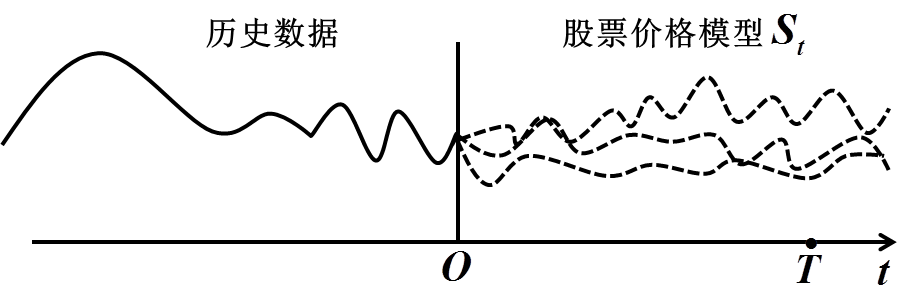
\includegraphics[width=6cm]{images/Contract_transaction.jpg}
		\caption{合同交易情况}
		\label{fig:合同交易情况}
		\end{figure}
		% \textcolor[rgb]{1 0 0 }{todo:图片:合同交易情况}。
		\par
		现在AB两人拟定这样一份合同:B可以在规定时刻$T$,用$k$元来购买股票(仅考虑1股)。如果股票在$T$时刻的价格$S_T$大于$k$ ($S_T>k$),则B购买股票,B赚${S_T}-k$,A赔${S_T}-k$。如果$S_T<k$,那么B不购买股票,B一点不赚,A一点不赔。很明显,这份合同对B是绝对有利的。所以在合同交易日$t=0$时刻,B只需要给A一定的钱$Y_0$(即合同价格)\footnote{注:期权价格:期望$T$时刻行使权利(合同)的价格,看涨期权即$S_T>k$。}。
		\par
		A要用合同约定的钱$Y_0$来把$T$时刻赔的钱$\max\{S_T-k,0\}$赚回来啊,而他能投资的对象是一种国债和一支股票(即A手中的唯一一支股票),二者的价格为:
		\begin{equation*}
			\centering
			\left\{\begin{lgathered}
			{\mathrm{d}{P_t} = {r_t} {P_t} \mathrm{d}t}\\
			{\mathrm{d}{S_t} = {b_t}{S_t}\mathrm{d}t + {\sigma _t}{S_t}\mathrm{d}{W_t}}\\
			{0 \leqslant t \leqslant T}\\
			{S\left( 0 \right) = {S_0}}
			\end{lgathered} \right.
		\end{equation*}
		\par
		A在$t=0$时刻用$Y_0$来投资,在$[0,T]$的$t$时刻,他的投资策略为$Y_t$中的$\pi_t$元来买股票,${Y_t}-{\pi_t}$来买债券,故其$Y_t$满足如下过程
		\begin{equation*}
			{\mathrm{d}{{Y_t}}} = \left[ {{r_t}{Y_t} + {\pi _t}\left( {{b_t} - {r_t}} \right)} \right]{\mathrm{d}t} + {\pi _t}  {\sigma _t} \mathrm{d}{}
		\end{equation*}
		令${\pi _t}{\sigma _t} = {Z_t}$,有
		\begin{align*}
			{\mathrm{d}}Y_t =[ {{r_t}{Y_t} +( {{b_t} - {r_t}})\sigma _t^{ - 1}{Z_t}}]{\mathrm{d}}t + Z_t{\mathrm{d}}W_t
		\end{align*}
		并且A要用$Y_t$来弥补$T$时刻亏损$\{{{S_T}-k},0\}$,即${Y_t}\geqslant \max \left\{ {{S_T} - k,0} \right\}$,但B又不会容许${Y_t} > \max \left\{ {{S_T} - k,0} \right\}$情况发生,故要求$Y_t$在$T$时刻价格等于$\max \left\{ {{S_T} - k,0} \right\}$。
		\begin{align}\label{eq:期权定价问题}
			\centering
			\left\{
			\begin{lgathered}
			{\mathrm{d}{Y_t} = [{r_t}{Y_t} + \left( {{b_t} - {r_t}} \right){\sigma _t}^{-1} {Z_t}]{\mathrm{d}t} + {Z_t}\mathrm{d}{W_t}}\\
			{\mathrm{d}{S_t} = {b_t}{S_t}\mathrm{d}t + {\sigma _t}{S_t}\mathrm{d}{W_t}}\\
			{{Y_t} = \max \left\{ {{S_T} - k,0} \right\}}\\
			{0 \leqslant t \leqslant T}\\
			{S\left( 0 \right) = {S_0}}
			\end{lgathered}
			 \right.
		\end{align}
		\par
		现在问题是:合同价格$Y_0$应该是多少,$Y_t,Z_t,S_t$是怎么确定的才能满足上面的要求。
		注:合同价格$Y_0$即为欧式看涨期权价格,上述问题也即期权定价问题,可以看到无论是前面的组合投资问题(\ref{eq:组合投资问题})还是后面的期权定价问题(\ref{eq:期权定价问题}),都是SDE终值问题。我们称式(\ref{eq:组合投资问题})为倒向随机微分方程(BSDE),式(\ref{eq:期权定价问题})为正倒向随机微分方程(FBSDE),因为式(\ref{eq:期权定价问题})与一个SDE组成方程组,故为FBSDE。

\section{倒向随机微分方程理论}

	\subsection{倒向随机微分方程的一般形式}
		下面,我们用上面的例子引出BSDE与FBSDE的一般形式,介绍线性BSDE和非线性BSDE,并将BSDE模型规范化。
		\subsubsection{线性BSDE}
			上面的模型(\ref{eq:组合投资问题})和模型(\ref{eq:期权定价问题})并非线性BSDE,但由前一章介绍的SDE,我们不难给出线性BSDE的一般形式
			\begin{equation*}
				\centering
				\left\{\begin{lgathered}
				{\mathrm{d}{Y_t} = f\left( {{Y_t},t} \right)\mathrm{d}t + g\left( {{Y_t},t} \right)\mathrm{d}{W_t}}\\
				{{Y_T} = \xi }
				\end{lgathered} \right.
			\end{equation*}
			其中:${0 \leqslant t \leqslant T}$,且$f,g$为${Y_t},t$的线性函数,例如:
			\begin{equation*}
				\centering
				\left\{\begin{lgathered}
				{f\left( {{Y_t},t} \right) = {a_t} + {b_t}{Y_t}}\\
				{g\left( {{Y_t},t} \right) = {c_t} + {d_t}{Y_t}}
				\end{lgathered} \right.
			\end{equation*}
			\par
			1973.Bismnt(法)\cite{1973.Bismnt}在研究随机最优控制问题时,为解释Pontryagin最大值原理中伴随过程的随机性时,引入了线性BSDE。之后,1979.Arbin、1978.kabanov、1995.Cadenilas和Karatzas都利用BSDE为P极大值原理做出贡献。1978.Bismut的两篇文章\cite{1978.Bismut2}\cite{1978.Bismut1}系统的介绍了线性BSDE问题。
		\subsubsection{非线性BSDE}
			根据前一章SDE的内容,我们可以给出非线性BSDE的一般形式
			\begin{equation*}
				\centering
				\left\{\begin{lgathered}
				{\mathrm{d}{Y_t} = f\left( {{Y_t},t} \right)\mathrm{d}t + g\left( {{Y_t},t} \right)\mathrm{d}{W_t}}\\
				{Y_T} = \xi \\
				0 \leqslant t \leqslant T
				\end{lgathered} \right.
			\end{equation*}
			其中,$f,g$为一般形式的映射。
			\par
			但是,上面的非线性BSDE的一般形式并非我们下面要讨论的。我们用组合投资问题(\ref{eq:组合投资问题})和期权定价问题(\ref{eq:期权定价问题})来引出如下非线性BSDE的一般形式
			\begin{equation*}
				\centering
				\left\{\begin{lgathered}
				{\mathrm{d}{Y_t} = f( {t,{Y_t},{Z_t}} )\mathrm{d}t + g( {t,{Y_t},{Z_t}} )\mathrm{d}t + {Z_t}\mathrm{d}{W_t}}\\
				{{Y_t} = \xi }\\
				{0 \leqslant t \leqslant T}
				\end{lgathered} \right.
			\end{equation*}
			\par
			非线性FBSDE的一般形式
				\begin{equation*}
				\centering
				\left\{\begin{lgathered}
				\mathrm{d}{X_t} = b\left( {t,{X_t},{Y_t},{Z_t}} \right)\mathrm{d}t + \sigma \left( {t,{X_t},{Y_t},{Z_t}} \right)\mathrm{d}{t_t}\\
				\mathrm{d}{Y_t} = f\left( {t,{X_t},{Y_t},{Z_t}} \right)\mathrm{d}t + {Z_t}\mathrm{d}{W_t}\\
				Y\left( T \right) = {Y_T} = \varphi \left( {{X_t},T} \right)\\
				X\left( 0 \right) = x
				\end{lgathered} \right.
				\end{equation*}
			这种非线性BSDE不仅要求解$Y_t$过程,还需要求解$Z_t$过程。

			下面,我们先讨论BSDE,然后再讨论FBSDE。我们考虑Pardoux和Peng给出的非线性BSDE形式
				\begin{align}\label{eq:非线性BSDE形式}
				\centering
				\left\{\begin{lgathered}
				{ - d{Y_t} = f\left( {t,{Y_t},{Z_t}} \right)\mathrm{d}t + g\left( {t,{Y_t},{Z_t}} \right)\mathrm{d}t - {Z_t}\mathrm{d}{W_t}}\\
				{{Y_t} = \xi }\\
				{0 \leqslant t \leqslant T}
				\end{lgathered} \right.
				\end{align}
			其等价的积分形式为(在$[t,T]$上积分)
			\begin{align*}
			Y_t = \xi + {\int_t^T {f({Y_s},{Z_s},s)\mathrm{d}s}} - {\int_t^T }{{Z_s}\mathrm{d}{W_s}} \end{align*}
			其中,$t \in [{0,T}]$。
			我们将上式(\ref{eq:非线性BSDE形式})的BSDE形式规范化:\ding{172}量的空间\ding{173}映射空间\ding{174}解域。
			\par
			$Y_t$为$m$维,即共有$m$个分量,$Y_t \in {R^m}$;$W_t$是$d$ 维Brown运动,$Z_t \in {R^{m\times d}}$,$f$为一映射,即${f({t,Y_t,Z_t})}:{\Omega  \times [0,T] \times {R^m} \times {R^{m \times d}} \to {R^m}}$。$(Y_t,Z_t)$是一对随机过程,就某时刻$t$而言,$(Y_t,Z_t)$为随机变量(后面要定义解空间-随机过程集合)。$ {Y_T} = \xi $是一随机变量,$\xi  \in {R^m}$,应可测且平方可积。
			\par
			由于上面是在概率的基础上进行研究的,设$(\Omega ; {\mathcal{F},P})$为一概率空间(完备)。
			${\mathcal {F}}_t=\sigma \{ {W_s}: 0 \leqslant s \leqslant t \} $是${W_s}$自然信息族,且所有的${P_{}}$零测集亦包含在${\mathcal{F}}_t$中,则$\{ {\mathcal{F}}_t \}$是由$\{ W_t \}$产生的$\sigma$代数流。\\
			记:在$T$时刻${\mathcal {F}}_T$可测且平方可积的随机变量$\xi $的集合为$L^2({{\mathcal {F}}_T};R^\times)$,${{\mathcal {F}}_T}$可测是指只有到$T$时刻才能确定的量,则模型(\ref{eq:非线性BSDE形式})末端时刻的取值情况为$Y_T = \xi\in L^2({{\mathcal {F}}_T};R^m)$。
			\par
			\textbf{现在讨论解$(Y_t,Z_t)$的可行域。} 如果一随机过程${Y_t}$,$\forall t \in [ {0,\infty }) $,$Y_t$是关于${{\mathcal {F}}_t}$可测的随机变量,则称$Y_t$在${{\mathcal {F}}_t}$是适应的。记在$[0,T]$上${{\mathcal {F}}_t}$适应的随机过程集合为${\phi}_1 $。
			\par
			如果一随机过程$Y_t$满足:
			\begin{align*}
			E\int_0^T {{{\left| {{Y_t}} \right|}^2}\mathrm{d}t < \infty }
			\end{align*}
			则$Y_t$在$[0,T]$上平方可积。
			记:在$[0,T]$上平方可积的随机过程集合为${\phi}_2 $。
			记:在$[0,T]$上${{\mathcal {F}}_t}$可测且平方可积的随机过程集合为$L_{\mathcal{F}} ^2\left( {0,T\left| R^\times \right.} \right) = {\phi _1} \cap {\phi _1} $,则$\left( {{Y_t},{Z_t}} \right) \in L_{\mathcal{F}} ^2\left( {0,T\left| {{R^m} \times {R^{m \times d}}} \right.} \right)$。\\
			注:1.可测就是可测,平方可积就是平方可积。
			2.$L_{\mathcal{F}} ^2\left( {0,T\left| R^\times \right.} \right)$是一个Hilbert空间。
			3.${L^2}\left( {{\mathcal{F}_t};{R^d}} \right) : E\left( | X_t |^2 \right)< \infty$,其中$X_t$是随机变量。
			4.$L_{{\mathcal{F}}_t}^2((0,T);R^d):E\int_0^T|\phi_t|^2\mathrm{d}t < \infty$,其中:$\phi_t$是随机过程。
			\par
			上面给出了各个量的空间和解域,但并没有详细讨论映射的形式(例:$f$可能是连续、有界或者导数连续有界),我们在具体的问题中进行具体的分析。下面,我们将给出BSDE解的存在唯一性以及一些比较定理。

	\subsection{解的存在唯一性}
		\par
		1990.Peng和Pardoux\cite{1990.Pardoux}给出了非线性BSDE,并证明其解的存在唯一性。1991.Peng\cite{1991.Peng}获得了非线性BSDE的非线性Feynman-Kac公式,使BSDE与PDE相关联。1992.Peng\cite{1992.Peng}进一步讨论了F-K公式。1993.Peng\cite{1993.Peng}在$f$满足局部L条件下得到解的存在唯一性。1997.Daring和Pardoux\cite{1997.Daring}在$f$关于$y_t$单调,关于$z_t$满足全局L条件下得到解的存在唯一性。关于BSDE理论与应用更详细的内容可以参考:1997.EI.Karoui,Peng,Ouenei\cite{1997.EI.Karoui}、1999.Ma\cite{1999.Ma}和2007.Pardoux\cite{2007.Pardoux}。
		\begin{theorem}[BSDE解存在唯一性]
			若$f$满足:\par
			1).$\forall (y,z) \in {R^m} \times {R^{m \times d}}$,$f( \cdot,{y,z} )$是$R^m$值的$\{\mathcal{F}_t\}$适应过程,且满足
			\begin{align*}
			\int_0^T {| {f( {s,\infty })|} \mathrm{d}s \in L_{\mathcal{F}}^2( {0,T;{R^m}} )\triangleq  H_{\mathcal{F}} ^2( {0,T;{R^m}} )}
			\end{align*}
			\par
			2).$f$关于$(y,z)$满足lipschitz条件 ,即$\exists C > 0$($C$为L常数),使得$\forall y,y_1 \in {R^m}$,$\forall z,z_1 \in {R^{m \times d}}$,有$|{f ( {t,y,z}) - f ( {t,y_1,z_1})} | \leqslant C ( { | {y - {y_1}} | + | {z - {z_1}} |})$
			\noindent 且终值$\xi \in L_{\mathcal{F}_T}^2 ( {0,T;{R^m}} ) $,则BSDE存在唯一适应解$(Y_t,Z_t)$,若解$(Y_t,Z_t)\in L_{\mathcal{F}}^2 ( {0,T;{R^m \times {R^{m \times d}}}} ) $,即$(Y_t,Z_t)$是$[0,T]$上关于${\mathcal {F}}_t$可测且平方可积的,则$(Y_t,Z_t)$称为BSDE 的$L^2$适应解。
		\end{theorem}
			注:Let $\xi \in L_{\mathcal {F}_T}^2( {0,T;{R^m}} )$ and Let $f:\Omega \times [{0,T}] \times {R^m} \times {R^{m \times d}} \to {R^m}$ , leqslant such that\\
			  1. $f(t,y,z)$ is progressively measurableqslant for all $(y,z)$;\\
			  2. $f( {t,0,0}) \in L_{\mathcal {F}}^2( {0,T;{R^m}} ) = H_{\mathcal {F}}^2( {0,T;{R^m}} )$;\\
			  3. f sabsfies a  uniform Lipschitz condrton in $(y,z)$.
		\par
		将上述存在唯一性应用到线性BSDE,有
		\begin{equation*}
			\centering
			\left\{\begin{lgathered}
			{ - \mathrm{d}{Y_t} = [ {{\phi _t} + {A_t}{Y_t} + {B_t}{Z_t}} ]\mathrm{d}t - {Z_t}\mathrm{d}{W_t}}\\
			{{Y_T} = \xi  \in {R^m}}\\
			{0 \leqslant t  \leqslant T}
			\end{lgathered} \right.
		\end{equation*}
		其中:${\phi _t},{Y_t},{A_t} \in L_{\mathcal {F}}^2( {0,T;{R^m}})$,${B_t},{Z_t} \in L_{\mathcal {F}}^2( {0,T;{R^{m \times d}}} )$ ,且$A_t,B_t$有界。
		\par
		如果上述线性BSDE如前,存在唯一解$(Y_t,Z_t)$,那么$Y_t$可以显式求解出来
		\begin{align*}
			Y_t = E\left[ \xi X_T +\int_t^T \phi _s X_s\mathrm{d}s\middle| \mathcal{F}_t \right] \quad a.s
		\end{align*}
		其中:$X_s$满足如下线性SDE
			\begin{equation*}
			\centering
			\left\{\begin{lgathered}
			{{X_s} = {A_s}{X_s}{\mathrm{d}s} + {B_s}{X_s}\mathrm{d}{W_s}}\\
			{t \leqslant s \leqslant T}\\
			{{X_t} = 1}
			\end{lgathered} \right.
			\end{equation*}

	\subsection{Feynman-Kac公式}
		\par
		前面,我们讨论的是${{Y_T} = \xi  \in {R^m}}$。现在不妨假设有另一随机变量${X_T} \in {R^n}$,可通过映射$\varphi ( {{X_T}}):{R^n} \rightarrow {R^m}$,那么终止条件可以变为:${Y_T} = \varphi ( {{X_T}} )$,在这种情况下给出Feynman-Kac公式。考虑如下BSDE的积分形式
		\begin{align*}
		{Y_t} = \varphi \left( {{X_T}} \right) + \int_t^T {f\left( {s,{Y_s},{Z_s}} \right){\mathrm{d}s} - } \int_t^T {{Z_s}\mathrm{d}{W_s}}
		\end{align*}
		其对应的微分形式为
		\begin{equation*}
			\centering
			\left\{\begin{lgathered}
			{ - \mathrm{d}{Y_t} = f\left( {t,{Y_t},{Z_t}} \right){\mathrm{d}t} - {Z_t}\mathrm{d}{W_t}}\\
			{Y\left( T \right) = {Y_T} = \varphi \left( {{X_T}} \right) = \xi }\\
			{0 \leqslant t \leqslant T}
			\end{lgathered} \right.
		\end{equation*}
		 若$(Y_t,Z_t)$是上述BSDE的$L^2$适应解(${{\mathcal {F}}_t}$适应且平方可积),则$(Y_t,Z_t)$可表示为
		\begin{equation*}
			\centering
			\left\{\begin{lgathered}
			{Y_t} = u( {t,{X_t}} )\\
			{Z_t} = {\nabla _x}u( {t,x} )\\
			\forall t \in [ 0,T]
			\end{lgathered} \right.
		\end{equation*}
		 其中,$u(t,x)$是如下拟线性PDE的光滑解,${\nabla _x}u$是$u$关于$x$的梯度。
		\begin{equation*}
			\centering
			\left\{\begin{lgathered}
			{\frac{{\partial u}}{{\partial t}} + {Lu} + f\left( {t,u} \right) = 0}\\
			{u\left( {x,T} \right) = \varphi \left( x \right)}\\
			{\left( {x,t} \right) \in {R^n} \times \left[ {0,T} \right]}
			\end{lgathered} \right.
		\end{equation*}
		其中:$L$是二阶梯度微分算子
		\begin{equation*}
			L = \frac{1}{2}\sum\limits_{i = 1}^n {\frac{{{\partial ^2}}}{{\partial x_i^2}}}
		\end{equation*}
		\par
		为简便,假设$f,\varphi$是有界光滑的,它们的导数是有界的。在此假设下,PDE存在唯一有界光滑解$u(t,x)$并且其导数也是有界的。
	\subsection{比较定理}
		\begin{theorem}[比较定理]
			设$(f^{1},{\xi ^{1}} \triangleq Y_T^{1} \triangleq \varphi ^{1}({X_T}) )$,$({f^2},{\xi ^2})$是两组BSDE的参量,$(Y_t^{1},Z_t^{1})$ ,$(Y_t^2,Z_t^2)$ 是两组BSDE的$L^2$适应解。如果\\
			1). $\xi^{1} \geqslant {\xi ^2}\quad a.s$;\\
			2).$f^{1}( {t,Y_t^2,Z_t^2} ) \geqslant {f^2}( {t,Y_t^2,Z_t^2} )\quad a.e\ a.s$\\
			则$\forall t \in [ 0,T]$,有$Y_t^{1} \geqslant Y_t^2\ a.e\ a.s$。
		\end{theorem}
		\begin{corollary}
		若$\xi \geqslant 0\ a.s.$,$f( {t,\infty }) \geqslant 0\ a.s$,则$Y_t \geqslant 0\ a.s$。
		\end{corollary}
		注:Let $(\xi_1,f^1)$ leqslant standard parmeters and let $(y_t^1,z_t^1)$ and $(y_t^2,z_t^2)$ leqslant tleqslant solutions to their corresponding BSDEs, Suppoleqslant that\\
		1. ${\xi ^{1} \geqslant {\xi ^2}} \quad a.s$;\\
		2. ${f^{1}}( {t,y_t^2,z_t^2}) \geqslant {f^2}( t,y_t^2,z_t^2 )\quad \mathrm{d}t \otimes \mathrm{d}P ,a.e$;\\
		3. ${f^2}\left( {t,Y_t^2,Z_t^2} \right) \leqslant L_F^2\left( {0,T;{R^m}} \right)$
		Then, $y_t^{1} \geqslant y_t^2$for all$t \in [ {0,T} ]\quad a.s$。
		其证明可参见:1992.Pardoux\cite{1992.Pardoux}和1992.Peng\cite{1992.Peng}。

\section{倒向随机微分方程数值方法}
	\par
	上面给出了非线性BSDE解存在唯一性,Feynman-Kac公式以及比较定理。下面,我们来介绍一些数值算法:
	\begin{enumerate}
	  \item Euler格式
	  \item $\theta$格式
	  \item 变分$\theta$格式
	  \item Adams格式
	\end{enumerate}

	\subsection{Euler格式}
		\subsubsection{Euler格式的导出}
			\par
			先在一维情况下对数值格式/方法进行说明。${Y_t} \in R$,$W_t$是一维Brown运动
					\begin{align}
					\centering
					{Y_t} = \varphi \left( {{X_T}} \right) + \int_t^T {f\left( {s,{Y_s},{Z_s}} \right){d_s} - } \int_t^T {{Z_s}\mathrm{d}{W_s}}
			 		\end{align}
			 其中,$\varphi ({X_T}) = \xi  \in L_{{\mathcal{F}}_T}^2(R)$。\\
			\ding{172}\textbf{时间划分}
			\par
			对时间区间$[0,T]$进行如下划分,记划分为$\tau$。
			\begin{align*}
			0 = {t_0} < {t_1} <  \cdots  < {t_N} = T
			\end{align*}
			令$\Delta {t_n} = {t_{n + 1}} - {t_n},n = 0,1, \cdots ,N - 1$。\\
				\begin{equation*}
					\centering
					\left\{
						\begin{lgathered}
						\Delta {t_n} = \max_{0 \leqslant n \leqslant N - 1} \Delta {t_n}\\
						\Delta W{_n} = W_{t_{n + 1}} - W_{t_n}
						\end{lgathered}
					\right.
				\end{equation*}
			 这里,不防来用$N$等划分$\tau^{N}$,则$\Delta t = \frac{{T - 0}}{N}$。\\
			 \ding{173}\textbf{Brown运动的离散化}
			 \par
			 考虑一个Benoulli序列$\left\{ {{\xi _n}} \right\}_{n = 1}^N$,${\xi _n}$是独立同分布的随机变量且取值有限,且$E{\xi _n} > 0,D{\xi _n} = 1$,并且有$\xi_0=0$。假设$\xi_n$取值$x_j(j=1,2,\cdots,l)$的概率为$p_j$,则由期望和方差可知
				\begin{equation*}
					\centering
					\left\{\begin{lgathered}
					{\sum\nolimits_j {{p_j}{x_j} = 0} }\\
					{\sum\nolimits_j {{p_j}x_j^2 = 1} }
					\end{lgathered} \right.
				\end{equation*}
			则在$[t_n,t_{n+1}]$时间段内$\Delta W_{t_n} = \sqrt {\Delta {t_n}} {\xi _n} = \sqrt {\Delta t} {\xi _n}$。故可以将Brown运动$W_t$\footnote{注:在每个时间段内,$W_{t_n}$以概率$p_j$增加$x_j$。}表示为
			 		\begin{equation*}
					\centering
					{W_t} \approx W_t^N = \sum\limits_{n = 0}^{\left[ {t/\Delta t} \right]} {\sqrt {\Delta {t_n}} {\xi _n}}  = \Delta t \sum\limits_{n = 1}^{\left[ {t/\Delta t} \right]} {{\xi _n}} \quad 0 \leqslant t \leqslant T
					\end{equation*}
			\par
			易见,当$N \rightarrow \infty $时,$W_t^N \rightarrow {W_t}, a.e.$,即$W_t^N$几乎处处收敛于$W_t$。
			定义由离散Brown运动$W_t^N$形式的自然信息族为${\mathcal {F}}_{t_n}^N = \sigma ( {{\xi _0},{\xi _1}, \cdots ,{\xi _n}} )$,则$n$趋向无穷时,有${\mathcal {F}}_n^N \to {\mathcal {F}}_{t_n}^N$。\\
			\ding{174}\textbf{终端$Y_T$的处理}
			\par
			如果终端${Y_T} = \xi  = \varphi ( {( {{W_t}} )_{0 \leqslant t \leqslant T}} )$,其中:$\phi:D_{[0,T]}\to R$且满足$L$条件,那么我们需要让终端近似值${\xi ^N} = \varphi ( {( {W_t^N})_{0 \leqslant t \leqslant T}} )$满足
			\par
			1:$\xi \in {L_{{\mathcal{F}}_T}}( R )$,${\xi ^N} \in {L_{{\mathcal{F}}_T^N}}( R )$,有
			  \begin{align*}
			  E{| \xi  |^2} + \sup_n E{| {{\xi ^n}} |^2} < \infty
			  \end{align*}
			  以及
			  \begin{align*}
			  \lim_{n \to \infty } E{\left| {\xi  - {\xi ^n}} \right|^2} = 0
			  \end{align*}
			  \par
			 2:${\sum\limits_{j = 0}^N {| {f( {{t_j},\infty } )} |} ^2}\Delta t$相对于$N$一致有界。\\
			\textcircled{4}\textbf{离散BSDE方程}
			\begin{align*}
			\mathrm{d}{Y_t} =  - f\left( {t,{Y_t},{Z_t}} \right)\mathrm{d}t + {Z_t}\mathrm{d}{W_t}
			\end{align*}
			上述方程两边在$[ {{t_n},{t_{n + 1}}} ]$上积分有
			 		\begin{equation*}
						\centering
						\int_{{t_n}}^{{t_{n + 1}}} {\mathrm{d}{Y_t} =  - \int_{{t_n}}^{{t_{n + 1}}} {f\left( {s,{Y_s},{Z_s}} \right)\mathrm{d}s}  + \int_{{t_n}}^{{t_{n + 1}}} {{Z_s}\mathrm{d}{W_s} } }
					\end{equation*}
			 \par
			 对上式的右端积分项有以下三种处理方式:\\
			1).
			$
			\int_{{t_n}}^{{t_{n + 1}}} {f\left( {s,{Y_s},{Z_s}} \right)\mathrm{d}s}  = f\left( {{t_n},{Y_{{t_n}}},{Y_{{t_n}}}} \right)\Delta {t}
			$\\
			2).
			$
			\int_{{t_n}}^{{t_{n + 1}}} {f( {s,{Y_s},{Z_s}} )\mathrm{d}s}  = f( t_{n+1},Y_{t_{n+1}},Z_{t_{n+1}} )\Delta {t}
			$\\
			3).
			$
			\int_{{t_n}}^{{t_{n + 1}}} {f( {s,{Y_s},{Z_s}} )\mathrm{d}s} = \theta f( t_n,Y_{t_n},Z_{t_n} )\Delta t  + ( {1 - \theta } )f( {t_{n + 1}},Y_{t_{n + 1}},Z_{t_{n + 1}} )\Delta t
			$\\
			所以我们会有三种Euler格式(SDE中成为显式、隐式和$\theta$格式)。我们以第三种处理方式来看(由于3是一种一般的情况,1和2是3的特殊)。由
			\begin{align*}
			{Y_{{t_{n + 1}}}} - {Y_{{t_n}}} =  - \int_{{t_n}}^{{t_{n + 1}}} {f\left( {s,{Y_s},{Z_s}} \right)\mathrm{d}s + } \int_{{t_n}}^{{t_{n + 1}}} {{Z_s}\mathrm{d}{W_s}}
			\end{align*}
			有
			\begin{align*}
			Y_{t_n} &= Y_{t_{n + 1}} +[ \theta f( t_n,Y_{t_n},Z_{t_n} ) + (1 - \theta )f( t_{n + 1},Y_{t_{n + 1}},Z_{t_{n + 1}} )]\Delta t - Z_{t_n} \xi _{n + 1} \sqrt{\Delta t}
			\end{align*}
			\par
			一般来说$Z(T)$只影响$T$时刻后$(Y_t,Z_t)$的值,不妨设$Z_T=0$,并且对一般离散BSDE而言,可积$Z$的计算较为困难,而且在证明数值解收敛值和稳定性时会遇到困难,所以下面我们考虑$f$不含$Z$或者只是$Z$的线性函数(可通过Girsanov变换将线性函数变为不包含$Z$的情况)。
				\begin{align*}
					\left\{
					\begin{aligned}
					&Y_{t_n} = Y_{t_{n + 1}} + [ \theta f( t_n,Y_{t_n},Z_{t_n} ) + ( 1 - \theta  )f( t_{n + 1},Y_{t_{n + 1}},Z_{t_{n + 1}} )]\Delta t - {Z_{{t_n}}} {\xi _{n + 1}} \sqrt {\Delta t} \\
					&{Y_T} = {\xi ^N}\\
					&{Z_T} = 0\\
					&n = N - 1,N - 2, \cdots ,1,0
			 		\end{aligned}
			 		\right.
			 	\end{align*}
			对上式两边取条件期望
			\begin{align*}
			E(Y_{t_n}| \mathcal{F}_n^N) &= E\bigl(Y_{t_{n + 1}}+[\theta f( t_n,Y_{t_n},Z_{t_n} ) + ( 1 - \theta  )f( t_{n + 1},Y_{t_{n + 1}},Z_{t_{n + 1}} )]\Delta t| \mathcal{F}_n^N\bigr) \\
			&\quad - E(Z_{t_n}\xi _{n + 1}\sqrt {\Delta t} | \mathcal{F}_n^N  )
			\end{align*}
			又因为${{Z_{t_n}}}$与${{\xi _{n + 1}}}$相互转换,所以
			\begin{align*}
			E\left(Z_{t_n}\xi _{n + 1}\sqrt {\Delta t} \bigl| \mathcal{F}_n^N  \right) = \sqrt {\Delta t} E\left( Z_{t_n}\bigl| \mathcal{F}_n^N \right)E\left(\xi _{n + 1}\bigl| \mathcal{F}_n^N  \right) = 0
			\end{align*}
			由此得到\textbf{Euler格式}为
			 	\begin{align*}
					\left\{
					\begin{aligned}
					&Y_{t_n} = E\Bigl( Y_{t_{n+1}}+ \bigl[\theta f(t_n,Y_{t_n})+  (1-\theta) f(t_{n+1},Y_{t_{n+1}})\bigr ]\Delta t\Bigl|\mathcal{F}_n^N \Bigr)\\
					&Z_{t_n} = E\biggl( \frac{Y_{t_{n+1}} -Y_{t_n}+ \bigl[\theta f(t_n,Y_{t_n})+  (1-\theta) f(t_{n+1},Y_{t_{n+1}})\bigr ] \Delta t }{\sqrt{\Delta t}\xi_{n+1}} \Bigl|\mathcal{F}_n^N \biggr)\\
					&Y_T = \xi^N\\
					&Z_T = 0
					\end{aligned}
					\right.
				\end{align*}
			当$\theta=1$,得到\textbf{左端Euler格式}为
					\begin{equation*}
					\centering
					\left\{\begin{lgathered}
					Y_{t_n} = E\left( Y_{t_{n + 1}}\bigl|\mathcal{F}_n^N  \right) + f( t_n,Y_{t_n} )\Delta t\\
					Z_{t_n} = E\left( \frac{Y_{t_{n + 1}} - Y_{t_n} + f( t_n,Y_{t_n} )}{\sqrt {\Delta t} \xi _{n + 1}}\bigl| \mathcal{F}_n^N  \right)\\
					Y_T = \xi ^N\\
					Z_T = 0
					\end{lgathered} \right.
					\end{equation*}
			再进行一次迭代求解
					\begin{equation*}
					\centering
					\left\{\begin{lgathered}
					Y_{t_n} = E( Y_{t_{n + 1}}| \mathcal{F}_n^N ) + \frac{1}{n}f( t_n,Y_{t_n} )\\
					Z_{t_n} = E\left( \frac{Y_{t_{n + 1}} - Y_{t_n} + \frac{1}{n}f( t_n,Y_{t_n} )}{\sqrt {\Delta t} \xi _{n + 1}}\Bigl| \mathcal{F}_n^N  \right)\\
					Y_T = \xi ^N\\
					Z_T = 0
					\end{lgathered} \right.
					\end{equation*}
			 当$\theta=0$时,得到\textbf{右端Euler格式}为
					\begin{equation*}
						\centering
					\left\{\begin{lgathered}
					Y_{t_n} = E\left( Y_{t_{n + 1}} + f( t_{n + 1},Y_{t_{n + 1}} )\Delta t| \mathcal{F}_n^N \right)\\
					Z_{t_n} = E\left( \frac{Y_{t_{n + 1}} - Y_{t_n} + f( t_{n + 1},Y_{t_{n + 1}} )}{\sqrt {\Delta t} \xi_{n + 1}}\Bigl| \mathcal{F}_n^N\right)\\
					Y_T = \xi ^N\\
					Z_T = 0
					\end{lgathered} \right.
					\end{equation*}
			假设$(Y_t,Z_t)$为原BSDE的$L^2$适应解,$(Y_t^N,Z_t^N)$为离散BSDE的之Euler格式解。下面,我们来介绍数值解的存在唯一性和误差估计。
			\par
			2002.Protter\cite{2002.Protter}给出了左端Euler格式。2004.zhang\cite{2004.zhang}给出了左端Euler格式的强0.5阶收敛结果。2006.Gobet\cite{2006.Gobet}将结果推广到$L^p$范数下的强0.5解收敛。2006.Peng\cite{2006.Peng}给出了右端Euler格式的收敛性。Euler格式用多项随机游动来近似Brown运动,使终端条件和一般并且容易实现。但是,这种计算只具有弱收敛性,且由于空间复杂度$(E)$随维度增加而变大,很难用于高维度BSDE问题。

		\subsubsection{离散BSDE解的存在唯一性}
			若${\xi}^N,f$满足:\\
			1).${\xi}^N$是${{\mathcal{F}}_N^N}$可测的。\\
			2).$\exists C>0$,$\forall y_1,y_2,z_1,z_2$及$k$,有
			\begin{align*}
			\left| {f\left( {t,y_1,{z_1}} \right) - f\left( {t,y_2,{z_2}} \right)} \right| \leqslant C\left( {\left| {{y_1} - {y_2}} \right| + \left| {{z_1} - {z_2}} \right|} \right)
			\end{align*}
			且\begin{align*}
			E\left( {\sum\limits_k {{{\left| {f\left( {{t_k},{y_k},{z_k}} \right)} \right|}^2}} } \right) < \infty
			\end{align*}
			则当$\alpha \Delta tC <1$时,离散BSDE的方程存在唯一解$(Y_t^N,Z_t^N)$\footnote{注:上式中$f$中的$z$可略去(即写为$f(t,y)$)}。
		\subsubsection{数值解的误差估计}
			当$\theta=\frac 12$时,利用2项随机游动逼近Brown运动,对足够小的$\Delta t$,足够大的$N$
			\begin{align*}
			\mathop {\sup }\limits_{0 \leqslant n \leqslant N} \left| {Y_{{t_n}}^N - {Y_{{t_n}}}} \right| \leqslant \frac{{R\left( {{e^L} - 1} \right)}}{{2N}}
			\end{align*}
			其中,$R$为$f$的界,$L$为$f$的Lipschitz常数。
			\begin{align*}
			\left|Z_{t_n}^N - Z_{t_n}\right|\leqslant \frac{R(e^L-1)(2+L/N)}{2\sqrt{N}} \left(\sqrt{\frac{p^3}{1-p}}+\sqrt{\frac{(1-p)^3}{p}} \right)
			\end{align*}
		\subsubsection{收敛性}
			% \par
			% 2004.zhang\cite{2004.Zhang}给出了左端Euler格式的强0.5阶收敛结果
			% \begin{align*}
			% \max_{n \leqslant N}\sup_{t\in [t_n,t_{n+1}]} E[|Y_{t_n}^N-Y_{t_n}|^2]+\sum_{n=0}^{N-1}\int_{t_n}^{t_{n+1}}E|Z_{t_n}^N-Z_t|^2\mathrm{d}t \leqslant C\frac{T}{N}
			% \end{align*}
			% 2006.Gobet, Labart\cite{2006.Gobet}将上述结论推广到$L^p$范数下的强0.5阶收敛
			% \begin{align*}
			% \left\{\max_{n \leqslant N} E|Y_{t_n}^N-Y_{t_n}|^p+ \left(E\left[\sum_{n=0}^{N-1}\int_{t_n}^{t_{n+1}}|Z_{t_n}^N-Z_t|^2\mathrm{d}t\right] \right)^\frac{p}{2}\right\}^\frac{1}{p}\leqslant k(T,x)\frac{1}{\sqrt{N}}
			% \end{align*}
			\par
			2006.Peng给出右端Euler格式的收敛性
			\begin{align*}
			E\left[ {\mathop {\sup }\limits_{0 \leqslant n \leqslant N} {{\left| {Y_{{t_n}}^N - {Y_{{t_n}}}} \right|}^2}{\rm{ + }}\int_0^T {{{\left| {Z_s^N - {Z_s}} \right|}^2}\mathrm{d}s} } \right] \rightarrow 0
			\end{align*}
			如果当$n \to \infty $时,${{\mathcal{F}}_n^N} \to {{\mathcal{F}}_{t_n}}$,$\xi ^N \to \xi$,则
			\begin{align*}
			&E\left[ {\left| {Y_{{t_n}}^N - {Y_{{t_n}}}} \right|} \right] \to 0\quad \forall {t_n}\\
			&\int_t^T {Z_t^NdW_t^N}  \to \int_t^T {{Z_t}\mathrm{d}{W_t}}
			\end{align*}
			\par
			回顾前面Brown运动的离散化,我们假设$\xi_n$是独立同分布的随机变量且取值有限,$E\xi_n =0$,$D\xi_n =1$,$\xi_0=0$,并且$\xi_n$可能取值为$x_j(j=1,2,\cdots,l)$,取$x_j$的概率为$p_j$。下面,我们来示范一下这种离散化:
			\par
			1).二项随机游动逼近Brown运动。当$\xi_n$只取2个值$x_1,x_2$且概率$P$取值$x_1$,$(1-p)$取值$x_2$,那么在$[t_n,t_{n+1}]$时间段内,Brown运动以概率$P$增加${\Delta t{x_1}}$,以概率$1-p$增加${\Delta t{x_2}}$,例如:$x_1=1,x_2=-1,p=0.5$。
			\par
			2).三项随机游动逼近Brown运动。当$\xi_n$取值为$x_1,x_2,x_3$,且以概率$p^2$取值$x_1$,以 概率$2p(1-p)$取值$x_2$,以$(1-p)^2$概率取值$x_3$,那么在$[t_n,t_{n+1}]$时间段内,Brown运动以概率$P^2$增加${\Delta t{x_1}}$,以概率$2p(1-p)$增加${\Delta t{x_2}}$,以概率$(1-p)^2$增加${\Delta t{x_3}}$。例如:$x_1=2,x_2=0,x_3=-2,p=0.5$。
			\par
			3).L项随机游动逼近Brown运动。类推1)和2)。

	\subsection{Theta格式}
		\subsubsection{半Theta格式}
			对$\forall(t,x) \in [0,T]\times R^d$,记$t$时刻从$x$出发的Brown运动:$W_{s}^{t,x}=x+W_s-W_t \quad (t\leq s\leq T)$且$W$ 为$d$维标准Brown运动;记$W_t^x=x+W_t (\text{即当}s=t \text{时})$,则有$W_T^x=x+W_T$,
			记${{\mathcal{F}}_s^{t,x}}=\sigma\{ N\cup  \sigma\{W_r^{tx},t\leq r \leq s \} \}$。
			${L_{{\mathcal{F}}_s^t}^2}(t,T;r^m)$为所有平方可积且$E\int_t^T {{{\left| {{Y_s}} \right|}^2}\mathrm{d}s < \infty } $且与$\{{\mathcal{F}}_s^{tx}\}$适应的$R^m$值的随机过程$\phi$的集合。
			\par
			考虑如下BSDE
					\begin{equation*}
					\centering
					\left\{\begin{lgathered}
					{{Y_t} = \varphi \left( {W_T^{t,x}} \right) + \int_t^T {f\left( {s,{Y_s},{Z_s}} \right)\mathrm{d}s - \int_t^T {{Z_s}\mathrm{d}{W_s}} } }\\
					{W_T^{t,x} = x + {W_T} - {W_t}}
					\end{lgathered} \right.
					\end{equation*}
			其中:$\varphi:R^d\rightarrow R^m$,$f:[0,T] \times R^m \times R^{m\times d}\rightarrow R^m$,假设$f$关于$y,z$ 满足全局L 条件,且$\int_0^T {\left| {f\left( {s,0,0} \right)} \right|\mathrm{d}s < \infty } $,那么BSDE存在唯一$\{{\mathcal{F}}_s^{t,x}\}$适应解$( {{Y_t},{Z_t}} ) \in L_{{\mathcal{F}_t}}^2 \times ( {0,T;{R^m} \times {R^{m \times d}}} )$。此外,对$1 \leqslant k \leqslant m$,若${f^k} \in C_b^{1,2,2},{\varphi ^k} \in C_b^{2 + \alpha }$,
			 那么由\textbf{Feynman-Kay}公式,有
					\begin{equation*}
					\centering
					\left\{\begin{lgathered}
					{{Y_s} = u\left( {s,W_s^{t,x}} \right)}\\
					{{Z_s} = {\nabla _x}u\left( {s,W_s^{t,x}} \right)}\\
					{\forall s \in \left[ {t,T} \right)}
					\end{lgathered} \right.
					\end{equation*}
			其中:$u(t,x)$是下面PDE的$C_b^{1,2}$经典解。
					\begin{equation*}
					\left\{\begin{lgathered}
					{\frac{{\partial {u^k}}}{{\partial t}} + \frac{1}{2}\sum\limits_{i = 1}^d {\frac{{{\partial ^2}{u^k}}}{{\partial {x^i}\partial {x^i}}}}  + {f^k}( {s,u,{\nabla _x}u} ) = 0}  \qquad  {s \in [ {t,T} ),x \in {R^d}}\\
					{{u^k}( {T,x} ) = {\varphi ^k}( x )}  \qquad {x \in {R^d}}
					\end{lgathered} \right.
					\end{equation*}
			其中:${\nabla_x}u$是$u$关于$x$的梯度。这里,我们假设:$f,\varphi$有界光滑,则其导数和有界,并且PDE有唯一光滑解$u(t,\infty)$且解的导数有界。
			\par
			2006.zhao\cite{2006.zhao}提出BSDE的$\theta$格式,该方法结合PDE数值解法的特点,并且在时间空间$(t,x)$上进行离散,用MC方法结合插值法来近似条件数学期望。2009.zhao\cite{2009.zhao}给出了$\theta$格式的误差估计。
			\par
			我们在$f$中不含$z$的情况下引出$\theta$格式\\
			\ding{172}\textbf{时间划分}
			\par
			对时间区间$[0,T]$划分为$N$段,记划分方法为$\tau$。
			\begin{align*}
			0=t_0<t_1<\cdots<t_N=T\end{align*}
			记:
					\begin{equation*}
					\centering
					\left\{\begin{lgathered}
					{\Delta {t_n} = {t_{n + 1}} - {t_n}}\\
					{\Delta t = \mathop {\max }\limits_n \Delta {t_n}}\\
					{\Delta {W_n} = W_{t_{n + 1}} - W_{t_n}}
					\end{lgathered} \right.
					\end{equation*}
			其中:$n=0,1,\cdots,N-1$。
			并且假设划分$\tau$有如下性质:
			\begin{align*}
			\frac{{\max \Delta {t_n}}}{{\min \Delta {t_n}}} \leqslant {C_0}\end{align*}
			其中:$C_0$是常数。
			注:不妨采用$N$等分的$\tau^{+}$,$\Delta t = \frac{T}{N}$。\\
			\ding{173}\textbf{离散BSDE方程}
			\begin{align*}
			\mathrm{d}{Y_t} =  - f\left( {t,{Y_t},{Z_t}} \right)\mathrm{d}{W_t} + {Z_t}\mathrm{d}{W_t}\end{align*}
			在$[t_n,t_{n+1}]$上积分有
			\begin{align}\label{eq:离散BSDE的积分}
			&{Y_{{t_n}}} = {Y_{{t_{n + 1}}}} + \int_{_{{t_n}}}^{_{{t_{n + 1}}}} {f\left( {s,{Y_s}} \right)\mathrm{d}s - } \int_{_{{t_n}}}^{_{{t_{n + 1}}}} {{Z_s}\mathrm{d}{W_s}} \\
			&n=N-1,N-2,\ldots,1,0 \notag
			\end{align}
			\ding{174}\textbf{求$(Y_{t_n},Z_{t_n})$迭代公式}\\
			\checkmark \textbf{求$Y_{t_n}$迭代公式}
			\par
			对上述方程两边取${{\mathcal{F}}_s^{t,x}}$的条件数学期望
			(为方便书写,记$E_s^{t,x}[\cdot]=E[\cdot|{\mathcal{F}_s^{t,x}}]$,$E_{s,t}^{x}[\cdot]=E[\cdot|{\mathcal{F}_s^{t,x}}]$),有
					\begin{align}\label{eq:条件数学期望}
					{Y_{{t_n}}} &= E_{{t_n}}^x\left[ {{Y_{{t_{n + 1}}}}} \right] + \int_{_{{t_n}}}^{_{{t_{n + 1}}}} {E_{{t_n}}^x\left[ {f\left( {s,{Y_s}} \right)} \right]\mathrm{d}s - \underbrace {\int_{_{{t_n}}}^{_{{t_{n + 1}}}} {E_{{t_n}}^x\left[ {{Z_s}} \right]\mathrm{d}{W_s}} }_{ = 0}} \notag \\
					&= E_{{t_n}}^x\left[ {{Y_{{t_{n + 1}}}}} \right] + \int_{_{{t_n}}}^{_{{t_{n + 1}}}} {E_{{t_n}}^x\left[ {f\left( {s,{Y_s}} \right)} \right]\mathrm{d}s}
					\end{align}
			可以发现,上式右边的积分函数是一个常数(而非随机),故可以对它使用积分方法:
					\begin{align}\label{eq:积分方法}
					\int_{{t_n}}^{{t_{n + 1}}} {E_{{t_n}}^x\left[ {f\left( {s,{Y_s}} \right)} \right]\mathrm{d}s = {\theta _1}\Delta {t_n}f\left( {{t_n},{Y_{{t_n}}}} \right) + \left( {1 - {\theta _1}} \right)\Delta {t_n}E_{{t_n}}^x\left[ {f\left( {{t_{n + 1}},{Y_{{t_{n + 1}}}}} \right)} \right] + R_y^n}
					\end{align}
			其中:$\theta_1 \in [0,1]$。
			$R_y^n$为$y$的截断误差项,定义其为:
			\begin{align*}
			R_y^n = \int_{{t_n}}^{{t_{n + 1}}} {E_{{t_n}}^x\left[ {f\left( {s,{Y_s}} \right)} \right]\mathrm{d}s - \left[ {{\theta _1}\Delta {t_n}f\left( {{t_n},{Y_{{t_n}}}} \right) + \left( {1 - {\theta _1}} \right)\Delta {t_n}E_{{t_n}}^x\left[ {f\left( {{t_{n + 1}},{Y_{{t_{n + 1}}}}} \right)} \right]} \right]} \end{align*}
			\par
			将上式(\ref{eq:积分方法})代入式(\ref{eq:条件数学期望}),并消去$R_y^n$可得到$Y_{t_n}$的迭代公式:
			\begin{align*}
			{Y_{{t_n}}} = E_{{t_n}}^x\left[ {{Y_{{t_{n + 1}}}}} \right] + {\theta _1}\Delta {t_n}f\left( {{t_n},{Y_{{t_n}}}} \right) + \left( {1 - {\theta _1}} \right)\Delta {t_n}E_{{t_n}}^x\left[ {f\left( {{t_{n + 1}},{Y_{{t_{n + 1}}}}} \right)} \right]\end{align*}
			\checkmark \textbf{求$Z_{t_n}$迭代公式}
			\par
			上面得到$Y_{t_n}$的迭代公式。下面,我们来求解$Z_{t_n}$的迭代公式。令$\Delta {W_s} = {W_s} - {W_{{t_n}}},(s \in [t_n,t_{n+1}])$,$\Delta {W_s}$是一个期望为0,标准差为$\sqrt {\Delta {t_n}} $的标准Brown运动。对式(\ref{eq:离散BSDE的积分})两边同乘$\Delta {W_{t_n}^\mathrm{T}}$,然后在方程两边取${{\mathcal{F}}_t^{t,x}}$的条件数学期望$ E_{{t_n}}^x\left[ \cdot \right]$。
					\begin{equation*}
					\begin{split}
					E_{{t_n}}^x\left[ {{Y_{{t_n}}} \Delta W_{{t_{n + 1}}}^\mathrm{T}} \right] = E_{{t_n}}^x\left[ {{Y_{{t_{n + 1}}}}  \Delta W_{{t_{n + 1}}}^\mathrm{T}} \right] & + \int_{_{{t_n}}}^{_{{t_{n + 1}}}} {E_{{t_n}}^x\left[ {f\left( {s,{Y_s}} \right)\Delta W_{{t_{n + 1}}}^\mathrm{T}} \right]\mathrm{d}s}\\  &- \int_{_{{t_n}}}^{_{{t_{n + 1}}}} {E_{{t_n}}^x\left[ {{Z_s} \Delta W_{{t_{n + 1}}}^\mathrm{T}} \right]\mathrm{d}{W_s}}
					\end{split}
					\end{equation*}
			由条件数学期望的性质及Ito等距公式,有
			\begin{align*}
			0 = E_{{t_n}}^x[ {{Y_{{t_{n + 1}}}}  \Delta W_{{t_{n + 1}}}^\mathrm{T}} ] + \int_{_{{t_n}}}^{_{{t_{n + 1}}}} {E_{{t_n}}^x[ {f( {s,{Y_s}} ) \Delta W_{s}^\mathrm{T}} ]\mathrm{d}s}  - \int_{_{{t_n}}}^{_{{t_{n + 1}}}} {E_{{t_n}}^x[ {{Z_s} } ]\mathrm{d}s}
			\end{align*}
			\par
			同样,可以发现上式右边的被积函数是常函数(而非随机),或者说积分是普通积分而非随机积分,故可以用一些积分公式
			\begin{align*}
			\int_{_{{t_n}}}^{_{{t_{n + 1}}}} {E_{{t_n}}^x[ {{Z_s}} ]\mathrm{d}s}  = {\theta _3}\Delta {t_n}E_{{t_n}}^x[ {{Z_{{t_n}}}} ] + ( {1 - {\theta _3}} )\Delta {t_n}E_{{t_n}}^x[ {{Z_{{t_{n + 1}}}}} ] + R_{{z_1}}^n
			\end{align*}


			\begin{align*}
			\int_{t_n} ^{t_{n + 1}}E_{t_n}^x [f(s,Y_s)\Delta W_s^{\mathrm{T}}]\mathrm{d}s &= \underline {\theta_2\Delta t_nE_{t_n}^x[f(t_n,Y_{t_n})\Delta W_{t_n}^{\mathrm{T}}]}_{ = 0}\\
			&\quad + (1-\theta_2) \Delta t_nE_{t_n}^x[f(t_{n+1},Y_{t_{n+1}})\cdot \Delta W_{t_{n+1}}^{\mathrm{T}}] + R_z2^n
			\end{align*}
					% \begin{equation*}
					% \begin{split}
					% \int_{t_n}^{t_{n + 1}} {E_{t_n}^x\left[ f\left( s,Y_s \right)\Delta W_s^\mathrm{T} \right]\mathrm{d}s &= \underbrace {\theta _2\Delta t_nE_{t_n}^x\left[ f\left( t_n,Y_{t_n} \right)\Delta W_{t_n}^\mathrm{T} \right]}_{ = 0}\\
					% &+ \left( 1 - \theta _2\right)\Delta t_nE_{t_n}^x\left[ f\left( t_{n + 1},Y_{t_{n + 1}} \right)\Delta W_{t_{n + 1}}^\mathrm{T}\right] + } R_{z_2}^n
					% \end{split}
					% \end{equation*}
			令$R_z^n=R_{z_1}^n+R_{z_2}^n$,故有
					\begin{equation*}
					\begin{split}
					0 &= E_{{t_n}}^x\left[ {{Y_{{t_{n + 1}}}}  \Delta W_{{t_{n + 1}}}^\mathrm{T}} \right] + \left( {1 - {\theta _2}} \right)\Delta {t_n}E_{{t_n}}^x\left[ {f\left( {{t_{n + 1}},{Y_{{t_{n + 1}}}}} \right)\Delta W_{{t_{n + 1}}}^\mathrm{T}} \right]\\
					& - \left\{ {{\theta _3}\Delta {t_n}\left[ {{Y_{{t_n}}}} \right] + \left( {1 - {\theta _3}} \right)\Delta {t_n}E_{{t_n}}^x\left[ {{Y_{{t_{n + 1}}}}} \right]} \right\} + R_z^n
					\end{split}
					\end{equation*}
			\par
			同样忽略$R_z^n$,我们可以得到$Z_{t_n}$的迭代公式。综上,有下面的\textbf{半$\theta$格式:}\\
			给定$Y_T=y^N$,对$n=N-1,N-2,\ldots,1,0$有
			\begin{align*}
			{Y_{{t_n}}} = E_{{t_n}}^x\left[ {{Y_{{t_{n + 1}}}}} \right] + {\theta _1}\Delta {t_n}f\left( {{t_n},{Y_{{t_n}}}} \right) + \left( {1 - {\theta _1}} \right)\Delta {t_n}E_{{t_n}}^x\left[ {f\left( {{t_{n + 1}},{Y_{{t_{n + 1}}}}} \right)} \right]\end{align*}
					\begin{equation*}
					\begin{split}
					0 &= E_{{t_n}}^x\left[ {{Y_{{t_{n + 1}}}} \Delta W_{{t_{n + 1}}}^\mathrm{T}} \right] + \left( {1 - {\theta _2}} \right)\Delta {t_n}E_{{t_n}}^x\left[ {f\left( {{t_{n + 1}},{Y_{{t_{n + 1}}}}} \right)\Delta W_{{t_{n + 1}}}^\mathrm{T}} \right] \\
			 		&\quad - \left\{ {{\theta _3}\Delta {t_n}E_{{t_n}}^x\left[ {{Z_{{t_n}}}} \right] + \left( {1 - {\theta _3}} \right)\Delta {t_n}E_{{t_n}}^x\left[ {{Z_{{t_{n + 1}}}}} \right]} \right\}
					\end{split}
					\end{equation*}
			其中:${\theta _1},{\theta _2},{\theta _3} \in [0,1]$。
		\subsubsection{半$\theta$格式的误差估计}
			\par
			下面,我们给出半$\theta$格式的误差估计,为了简单,仅给出一维BSDE$(m=d=1)$的情况。
			定义$(Y_{t_n}^N,Z_{t_n}^N)$为半$\theta$格式的解,$(Y_{t_n},Z_{t_n})$为BSDE的解。\\
			\noindent (1)若$f \in C_b^{1,3},\varphi \in C_b^{3+\alpha}$,则对$\theta_1,\theta_2 \in [0,1]$,$\theta_3 \in (0,1]$,有
					\begin{align*}
					{\left| {R_y^n} \right| \leqslant C{{\left( {\Delta {t_n}} \right)}^2}}\\
					{\left| {R_z^n} \right| \leqslant C{{\left( {\Delta {t_n}} \right)}^2}}
					\end{align*}
			 \noindent (2)若$f \in C_b^{2,5},\varphi \in C_b^{5+\alpha}$,则对$\theta_1=\theta_2 =\theta_3 =\frac 12$,有
					\begin{align*}
					{\left| {R_y^n} \right| \leqslant C{{\left( {\Delta {t_n}} \right)}^3}}\\
					{\left| {R_z^n} \right| \leqslant C{{\left( {\Delta {t_n}} \right)}^3}}
					\end{align*}
			 其中:$C$是依赖于$T$和$f,\varphi,u$导数上界的正常数,$u$为PDE的经典解。%%%%%字母不一定对
		\subsubsection{半$\theta$格式的收敛性}
			我们还给出$e_y^n=Y_{t_n}^N-Y_{t_n}$,$e_z^n=|{Z_{t_n}^N}-{Z_{t_n}}|$的$L^{1}$估计。\\
			\noindent (1)若$f \in C_b^{1,3},\varphi \in C_b^{3+\alpha}$,则对给出的$\forall t_n,\forall \theta_1\in [0,1]$,都有
			\begin{align*}
			\mathop {\max }\limits_{0 \leqslant n \leqslant N}E|Y_{t_n}^N-Y_{t_n}| \leqslant C\Delta {t} \end{align*}
			 \noindent (2)若$f \in C_b^{2,5},\varphi \in C_b^{5+\alpha}$,那么对足够小的$\Delta {t}$和$\theta_1=\frac 12$,有
			\begin{align*}
			{\mathop {\max }\limits_{0 \leqslant n \leqslant N}}E|Y_{t_n}^N-Y_{t_n}| \leqslant C(\Delta {t})^2 \end{align*}
			 \noindent (3)若$f \in C_b^{2,5},\varphi \in C_b^{5+\alpha}$,那么对足够小的$\Delta {t}$和$\theta_1=\frac 12,\theta \in [0,1],\theta_s=1$,有
			\begin{align*}
			\mathop {\max }\limits_{0 \leqslant n \leqslant {N-1}}E|Z_{t_n}^N-Z_{t_n}| \leqslant C\Delta {t} \end{align*}
			其中:$C$是依赖于$T$和$f,\varphi,u$导数上界的正常数。\\
			注:当$\theta_1 = \theta_2 = \theta_3 = 1$时,为左端Euler格式;当$\theta_1 = \theta_2 = \theta_3 = 0$时,为右端Euler格式;当$\theta_1 = \theta_2 = \theta_3 = \frac{1}{2}$时,为Crank - Nicolson。
		\subsubsection{全$\theta$格式}
			为简便仅考虑$m=d=1$的情况,$W_s^{tx}=x+W_s-W_t(t \leqslant s \leqslant T) ,(t,x)\in [0,T] \times R$。上面的半$\theta$格式是时间$t$方向上的离散格式,我们还可以做一个空间$X$上的离散,称这种时间$t$空间$X$上的离散为全$\theta$格式。记$x \in R$的全空间的一个划分为$\mathcal{R}_h$
			\begin{align*}
			\mathcal{R}_h = \{x_i|x_i\in R,i\in \mathbb{Z},x_i<x_{i+1},\lim_{i\to \infty} x_i =\infty ,\lim_{i\to -\infty} x_i =-\infty\}
			\end{align*}
			其中,$\mathbb{Z}$为整数集,$x_i$都是确定的。
			记$\Delta {x}_i=x_{i+1}-x_{i}$,$\Delta {x}={\mathop {\max }\limits_{i \in \mathbb{Z}} }\Delta {x}_i$
			\par
			$(Y_t,Z_t)$为BSDE的解析解。其在$(t_n,x_i)$点处的值的近似解(数值解)为$Y_i^n$,则有\textbf{全$\theta$格式}:
			给定$Y_i^N(i \in \mathbb{Z})$,寻找$(Y_i^n,Z_i^n) (i \in \mathbb{Z},n=N-1,N-2,\ldots,1,0)$,有
					\begin{equation*}
					Y_i^n = \hat E_{{t_n}}^{{x_i}}\left[ {{{\hat Y}^{n + 1}}} \right] + {\theta _1}\Delta {t_n}f\left( {{t_n},Y_i^n} \right) + \left( {1 - {\theta _1}} \right)\Delta {t_n}\hat E_{{t_n}}^{{x_i}}\left[ {f\left( {{t_{n + 1}},{{\hat Y}^{n + 1}}} \right)} \right]
					\end{equation*}
							\begin{equation*}
							\begin{split}
						0 = \hat E_{{t_n}}^{{x_i}}\left[ {{{\hat Y}^{n + 1}} \Delta {W_{n + 1}}} \right] &+ \left( {1 - {\theta _2}} \right)\Delta {t_n}\hat E_{{t_n}}^{{x_i}}\left[ {f\left( {{t_{n + 1}},{{\hat Y}^{n + 1}}} \right)  \Delta {W_{n + 1}}} \right]\\
						&- \left\{ {{\theta _3}\Delta {t_n}\hat E_{{t_n}}^{{x_i}}\left[ {Z_t^n} \right] + \left( {1 - {\theta _3}} \right)\Delta {t_n}\hat E_{{t_n}}^{{x_i}}\left[ {{{\hat Z}^{n + 1}}} \right]} \right\}
							\end{split}
							\end{equation*}
			其中:${\hat Y}^{n + 1}$,${\hat Z}^{n + 1}$分别是${Y}_l^{n + 1}$和${z}_l^{n + 1},l \in \mathbb{Z}$在空间点$W_{{t_{n + 1}}}^{{t_n},{x_i}} = {x_i} + {W_{{t_{n + 1}}}} - {W_{{t_n}}}$处的插值;$\hat E_{{t_n}}^{{x_i}}\left[ \cdot \right]$是$ E_{{t_n}}^{{x_i}}\left[ \cdot \right]$的近似解,可以用\textbf{MC}方法或者\textbf{Gauss-Hermite}方法来实现。\\
			注:MC方法常被用于计算数学期望,条件数学期望(积分), 但因为MC近似收敛于的值与$\frac {1}{\sqrt{M}}$成正比,用MC方法要消耗大量的时间,所以在实际中较多采用\textbf{Gauss-Hermite}积分公式。
			\par
			\begin{definition}[Gauss-Hermite积分公式]
				 \par
				 给定一个一维光滑函数$\rho(x)$,其Gauss-Hermite积分公式为
				 \begin{align*}
				 \int_{ - \infty }^{ + \infty } {{e^{ - {x^2}}}\rho \left( x \right)\mathrm{d}x}  \approx \sum\limits_{i = 1}^k {{w_i}\rho \left( {{\eta_i}} \right)}
				 \end{align*}
				 其中:$\eta_i$是如下$k$阶Hermite多项式的$k$个根
				 \begin{align*}
				 {H_k}\left( x \right) = {\left( { - 1} \right)^k}{e^{{x^2}}}\frac{{{\mathrm{d}^k}}}{{\mathrm{d}{x^k}}}\left( {{e^{ - {x^2}}}} \right)
				 \end{align*}
				 $w_i$是权重,由下式确定
				 \begin{align*}
				 {w_i} = \frac{{{2^{k + 1}}k!\sqrt \pi  }}{{{{\left[ {H_k'\left( {{\eta _i}} \right)} \right]}^2}}}
				 \end{align*}
				截断误差项$R(\rho,k)$为\\
				\begin{align*}
				R\left( {\rho ,k} \right) = \int_{ - \infty }^{ + \infty } {{e^{ - {x^2}}}\rho \left( x \right)\mathrm{d}x}  - \sum\limits_{i = 1}^k {{w_i}\rho \left( {{\eta_i}} \right)}
				\end{align*}
				且$\exists v \in R$使得$R\left( {\rho ,k} \right) = \frac{{k!\sqrt \pi  }}{{{2^k}\left( {2k} \right)!}}{\rho ^{2k}}\left( v \right)$。
			\end{definition}
			\par
			由\textbf{Gauss-Hermite}积分公式我们给出$ E_{{t_n}}^{{x_i}}\left[ \cdot \right]$的估计值$\hat E_{{t_n}}^{{x_i}}\left[ \cdot \right]$的计算公式
			\begin{align*}
					&\hat E_{{t_n}}^{{x_i}}\left[ {{{\hat Y}^{n + 1}}} \right] = \frac{1}{{\sqrt \pi}}\sum\limits_{j = 1}^k {{w_j}{I_h}{Y^{n + 1}}\left( {{x_i} + \sqrt {2\Delta {t_n}}  {\eta _j}} \right)} \\
					&\hat E_{{t_n}}^{{x_i}}\left[ {{{\hat Z}^{n + 1}}} \right] = \frac{1}{{\sqrt \pi  }}\sum\limits_{j = 1}^k {{w_j}{I_h}{Z^{n + 1}}\left( {{x_i} + \sqrt {2\Delta {t_n}} {\eta _j}} \right)} \\
					&\hat E_{{t_n}}^{{x_i}}\left[ {f\left( {{t_{n + 1}},{{\hat Y}^{n + 1}}} \right)} \right] = \frac{1}{{\sqrt \pi  }}\sum\limits_{j = 1}^k {{w_j}f\left( {{t_{n + 1}},{I_h}{Y^{n + 1}}\left( {{x_i} + \sqrt {2\Delta {t_n}} {\eta _j}} \right)} \right)} \\
					&\hat E_{{t_n}}^{{x_i}}\left[ {f\left( {{t_{n + 1}},{I_h}{{\hat Y}^{n + 1}}} \right)\Delta {W_{{t_{n + 1}}}}} \right] = \frac{1}{{\sqrt \pi  }}\sum\limits_{j = 1}^k {{w_j}f\left( {{t_{n + 1}},{I_h}{Y^{n + 1}}\left( {{x_i} + \sqrt {2\Delta {t_n}} {\eta_j}} \right)} \right)} \left( {\sqrt {2\Delta {t_n}}   {\eta_j}} \right)
			\end{align*}
			 其中:${{I_h}{Y^{n + 1}}\left( {{x_i} + \sqrt {2\Delta {t_n}}  {\eta _j}} \right)}$是$Y_{l}^{n + 1}(l \in \mathbb{Z})$在$x_i+\sqrt {2\Delta {t_n}} {\eta _j}$附近插值得到的${Y^{n + 1}}\left( {{x_i} + \sqrt {2\Delta {t_n}} {\eta _j}} \right)$的近似值。
		\subsubsection{全$\theta$格式的误差估计}
			设$(Y_i,Z_i)$是BSDE的解,$(Y_i^n,Z_i^n)$是全$\theta$格式的解,则当$\Delta {t}$和$\Delta {x}$足够小时,对$\theta \in [0,1]$,有
			\begin{align*}
			\mathop {\max }\limits_{i,n} \left| {Y_{{t_n}}^{{x_i}} - Y_i^n} \right| \leqslant C\left( {\Delta t + \frac{{{{\left( {\Delta x} \right)}^2}}}{{\Delta t}} + \frac{{k!}}{{\Delta t{2^k}\left( {2k} \right)!}}} \right)\end{align*}
			特别地,当$\theta=\frac 12$时,有
			\begin{align*}
			\mathop {\max }\limits_{i,n} \left| {Y_{{t_n}}^{{x_i}} - Y_i^n} \right| \leqslant C\left( {(\Delta t )^2+ \frac{{{{\left( {\Delta x} \right)}^2}}}{{\Delta t}} + \frac{{k!}}{{\Delta t{2^k}\left( {2k} \right)!}}} \right)\end{align*}
			 当$\theta=1$时,有
			 \begin{align*}
			 \mathop {\max }\limits_{i,n} \left| {Z_{{t_n}}^{{x_i}} - Z_i^n} \right| \leqslant C\left( {\Delta t + \frac{{{{\left( {\Delta x} \right)}^2}}}{{\Delta t}} + \frac{{k!}}{{\Delta t{2^k}\left( {2k} \right)!}}} \right)\end{align*}

	\subsection{变分Theta格式}
		\par
		前面介绍了Euler格式和$\theta$格式。下面将介绍另一种数值方法—变分$\theta$格式。我们先来考虑变分半$\theta$格式及其误差估计,然后给出变分全$\theta$格式。
		\subsubsection{变分半$\theta$格式}
			变分半$\theta$格式和半$\theta$格式相同的是:时间划分$\tau $和$Y_{t_n}$的迭代公式,不同的是$Z_{t_n}$的迭代公式。\\
			 \ding{172}\textbf{时间划分$\tau$}\\
			 \ding{173}\textbf{离散BSDE方程}\\
			 \ding{174}\textbf{求$Y_{t_n},Z_{t_n}$迭代公式}\\
			\checkmark \textbf{求$Y_{t_n}$迭代公式}
			 \begin{align*}
			 {Y_{{t_n}}} = E_{{t_n}}^x\left[ {{Y_{{t_{n + 1}}}}} \right] + {\theta _1}\Delta {t_n}f\left( {{t_n},{Y_{{t_n}}}} \right) + \left( {1 - {\theta _1}} \right)\Delta {t_n}E_{{t_n}}^x\left[ {f\left( {{t_{n + 1}},{Y_{{t_{n + 1}}}}} \right)} \right]
			 \end{align*}
			\checkmark \textbf{求$Z_{t_n}$迭代公式}
			\par
			为了得到$Z$的高阶近似,我们引入BSDE的变分方程(2002.Ma,zhang\cite{2002.Ma})。
			对$k=1,2,\ldots,m  (Y_t \in R^m) ,j=1,2,\ldots,d$($W_t$是$d$维Brown运动)
					\begin{align}\label{eq:1}
					{\nabla _j}Y_s^k = {\partial _x}{\varphi ^k}\left( {W_T^{tx}} \right){e_j} + \int_s^T {{\partial _y}{f^k}\left( {r,{Y_r}} \right){\nabla _j}{Y_r}\mathrm{d}r}  - \int_s^T {{\nabla _j}Z_r^k\mathrm{d}{W_r}} \quad s \in [t,T]
					\end{align}
			其中:${e _j}=(0,\ldots,0,1,0,\ldots,0)^T$是$R^d$中第$j$个坐标向量;
			\par
			$Z^{k,:}=(Z^{k-1},\ldots,Z^{k-d})$是$n \times d$维矩阵$Z$的第$k$行;
			\par
			${\partial _x}{\varphi ^k} = \left( {\partial_{x^1}{\varphi ^k}, \ldots ,\partial_{x^d}{\varphi ^k}} \right)$是$\varphi^k$ 关于$x\in R^d$的梯度,$x=(x^1,x^2,\ldots,x^d)^\mathrm{T}$;\par
			${\partial _x}{f ^k} = \left( {\partial_{x^1}{f ^k}, \ldots ,\partial_{x^d}{f ^k}} \right)$ ;
			\par
			$W_s^{t,x}=x+W_s-W_t(t \leqslant s \leqslant T)$是$t$时刻从$x$出发的Brown运动;
			\par
			${\nabla _j}Y_s^k$是一随机过程,是$Y_s^k$关于$x^j$的变分;
			\par
			${\nabla_j}Z_s^{k,i}$是一随机过程,是$Z_s^k$关于$x^j$的变分。
			\par
			将上式写成矩阵的形式有
			 \begin{align*}
			 \nabla {Y_t} = {\varphi _x '}\left( {W_T^{t,x}} \right) + \int_t^T {f_y '\left( {s,{Y_s}} \right)} \nabla {Y_s}\mathrm{d}s - \int_t^T {\nabla {Z_s}\mathrm{d}{W_s}} \end{align*}
			由$\forall s \in [0,T)$
			 ,${Y_s} = u\left( {s,W_s^{t,x}} \right)$,${Z_s} = {\nabla _x}u\left( {s,W_s^{t,x}} \right)$,我们有:${Z_t} = \nabla {Y_t}$,即
			\begin{align}\label{eq:2}
			Z_s^{k,j} = {\nabla _j}Y_s^k \quad s \in [t,T)
			\end{align}
			将式(\ref{eq:2})代入式(\ref{eq:1}),有
			\begin{align*}
			Z_s^{k,j} = {\partial _x}{\varphi ^k}( {W_T^{t,x}} ){e_j} + \int_s^T {{\partial _y}{f^k}( {r,{Y_r}} )} Z_r^{i,j}\mathrm{d}r - \int_t^T {{\nabla _j}Z_r^{i,k}\mathrm{d}{W_r}} \quad s \in [t,T]
			\end{align*}
			其中:$Z^{:,j}$是$m \times d$维矩阵$Z$的第$j$列。
			\par
			写出上式的离散方程,有
			\begin{align}\label{eq:3}
			Z_{{t_n}}^{k,j} = Z_{{t_{n + 1}}}^{k,j} + \int_{{t_n}}^{{t_{n + 1}}} {{\partial _y}{f^k}\left( {s,{Y_s}} \right)Z_s^{:,j}\mathrm{d}s}  - \int_{{t_n}}^{{t_{n + 1}}} {{\nabla _j}Z_r^{k,:}\mathrm{d}{W_s}}
			\end{align}
			对上式两边取条件数学期望$E_{{t_n}}^x[\cdot]$,有
			\begin{align*}
			Z_{{t_n}}^{k,j} = E_{{t_n}}^x\left[ {Z_{{t_{n + 1}}}^{k,j}} \right] + \int_{{t_n}}^{{t_{n + 1}}} {E_{{t_n}}^x\left[ {{\partial _y}{f^k}\left( {s,{Y_s}} \right)Z_s^{:,j}\mathrm{d}s} \right]}
			\end{align*}
			即\begin{align*}
			Z_{t_n} = E_{t_n}^x[Z_{t_{n + 1}}] + \int_{t_n}^{t_{n + 1}}E_{t_n}^x\left[{\partial _y}{f^k}(s,Y_s)Z_s\mathrm{d}s\right]
			\end{align*}
			同样上式的右端积分项为常积分,用$\theta$方法近似积分,并记截断误差项为$R_2^n$
			\begin{align*}
			Z_{t_n} = E_{t_n}^x[ Z_{t_{n + 1}} ] + \theta _2\Delta {t_n}{\partial _y}f( t_n,Y_{t_n} )Z_{t_n} + ( 1 - {\theta _2} )\Delta {t_n}E_{t_n}^x[ {\partial _y}f(t_{n + 1},Y_{t_{n + 1}})Z_{t_{n + 1}}]
			\end{align*}
			综上,有\textbf{变分半$\theta$格式}:
			对$1\leqslant k \leqslant m$, $1\leqslant j \leqslant d$,给定$Y^N,Z^N$,有
			\begin{align*}
			&Y_{t_n} = E_{t_n}^x[Y_{t_{n+1}}] + {\theta _1}\Delta {t_n}f(t_n,Y_{t_n})+(1-{\theta _1})\Delta {t_n}E_{t_n}^x[f(t_{n + 1},Y_{t_{n + 1}})] \\
			&Z_{t_n} = E_{t_n}^x[Z_{t_{n + 1}}] + {\theta _2}\Delta {t_n}{\partial _y}f(t_n,Y_{t_n})Z_{t_n} + (1-{\theta _2})\Delta {t_n}E_{t_n}^x[{\partial _y}f(t_{n + 1},Y_{t_{n + 1}})Z_{t_{n + 1}}]
			\end{align*}
			\par
			将上面的格式写为分量形式,有
				\begin{align*}
					&Y_{t_n}^k = E_{t_n}^x\left[Y_{t_{n + 1}}^k\right] + {\theta _1}\Delta {t_n}{f^k}\left(t_n,Y_{t_n}\right) + \left(1 - {\theta _1}\right)\Delta {t_n}E_{t_n}^x[f^k\left(t_{n + 1},Y_{t_{n + 1}}\right)]\\
					&Z_{t_n}^{k,j} = E_{t_n}^x\left[Z_{t_{n + 1}}^{k,j}\right] + {\theta _2}\Delta {t_n}\partial y{f^k}\left(t_n,Y_{t_n}\right)Z_{t_n}^{k,j} + \left(1 - {\theta _2} \right)\Delta {t_n}E_{t_n}^x\left[\partial yf^k\left(t_{n + 1},Y_{t_{n + 1}}\right)Z_{t_n}^{:,j} \right]
				\end{align*}
			其中:
			\begin{align*}
			R_2^n = \left(R_2^{k,j,n}\right)_{m \times d}
			\end{align*}
		\subsubsection{变分半$\theta$格式的误差估计}
			对$1 \leqslant k \leqslant m,1 \leqslant j \leqslant d$,$R_y^{k,n}$与$R_2^{k,j,n}$是截距误差项\\
			\noindent (1)若$f^{k} \in C_b^{1,3},{\varphi}^k \in C_b^{3+\alpha}$,则对$\theta_1,\theta_2 \in [0,1]$,有
					\begin{equation*}
						\centering
					\left\{\begin{lgathered}
					{\left| {R_y^{k,n}} \right| \leqslant C{{\left( {\Delta {t_n}} \right)}^2}}\\
					{\left| {R_z^{k,j,n}} \right| \leqslant C{{\left( {\Delta {t_n}} \right)}^2}}
					\end{lgathered} \right.
					\end{equation*}
			\noindent (2)若$f^{k} \in C_b^{2,5},{\varphi}^k  \in C_b^{5+\alpha}$,则对$\theta_1=\theta_2 =\frac 12$,有
					\begin{equation*}
						\centering
					\left\{\begin{lgathered}
					{\left| {R_y^{k,n}} \right| \leqslant C{{\left( {\Delta {t_n}} \right)}^3}}\\
					{\left| {R_z^{k,j,n}} \right| \leqslant C{{\left( {\Delta {t_n}} \right)}^3}}
					\end{lgathered} \right.
					\end{equation*}
			 其中:$C$是依赖于$m,d,T$和$f,\varphi,u$导数上界的正常数,$u$为PDE的经典解。
			 \par
			 令$(Y_t,Z_t)$是BSDE的解析解,$(Y_t^N,Z_t^N)$是变分半$\theta$格式的解\\
			 \noindent (1)若$f^{k} \in C_b^{1,3},{\varphi}^k \in C_b^{3+\alpha}$,则对对足够小的$\Delta {t}$和$ \theta_1 \theta_2\in [0,1]$,都有
			\begin{align*}
			\mathop {\max }\limits_{0 \leqslant n \leqslant N}E{|Y_{t_n}^N-Y_{t_n}|}^2 \leqslant C{\Delta {t}}^2 \\
			\mathop {\max }\limits_{0 \leqslant n \leqslant N}E{|Z_{t_n}^N-Z_{t_n}|}^2 \leqslant C{\Delta {t}}^2 \end{align*}
			 \noindent (2)若$f^{k} \in C_b^{2,5},{\varphi}^k\in C_b^{5+\alpha}$,那么对足够小的$\Delta {t}$和$\theta_1=\theta_2=\frac 12$,有
			\begin{align*}
			\mathop {\max }\limits_{0 \leqslant n \leqslant N}E{|Y_{t_n}^N-Y_{t_n}|}^2 \leqslant C{\Delta {t}}^4 \\
			\mathop {\max }\limits_{0 \leqslant n \leqslant N}E{|Z_{t_n}^N-Z_{t_n}|}^2 \leqslant C{\Delta {t}}^4
			\end{align*}
			 其中:$C$是一个依赖于$C_0,m,d,T$和$f,\varphi,u$导数上界的正常数,$u$为PDE的经典解。\\
			注:易给出变分全$\theta$格式,这里不再介绍。2012.zhao\cite{2012.zhao}提出了新的更一般的$Theta$格式。

	\subsection{多步Adams格式}

		2010.zhao\cite{2010.zhao}提出一种多步格式。前面介绍的Euler格式,$\theta$格式和变分$\theta$格式都是单步算法,即为求$Y_{t_n}$,只要用$Y_{t_{n+1}}$ 即可。为了提高截断误差项的阶数,在每个时间步$[t_n,t_{n+1}]$必须增加$E_{t_n}^x[f(t,y)]$的总次数,这样会无疑会增大计算量。
		\par
		下面,我们将介绍一种线性多步算法—Adams格式,为求$Y_{t_n}$,我们需要用$Y_{t_{n+1}},Y_{t_{n+2}},\ldots,Y_{t_{n+m}}$ 来计算,且每进行一步,只计算一次$E_{t_n}^x[f(t,y)]$的值。
		\subsubsection{半Adams格式:仅考虑时间离散}
		像前面的半$\theta$格式和全$\theta $格式那样,我们先给出半Adams格式。\\
			\ding{172}\textbf{时间离散划分$\tau$}\\
			\ding{173}\textbf{离散BSDE}\\
			\ding{174}\textbf{求$(Y_{t_n},Z_{t_n})$迭代公式}\\
			\checkmark \textbf{求$Y_{t_n}$迭代公式}
			\par
			假设我们已经知道了$(Y_{t_{n+1}},Z_{t_{n+1}}),(Y_{t_{n+2}},Z_{t_{n+2}}),\ldots,(Y_{t_{n+m}},Z_{t_{n+m}})$ 的值,则对$0 \leqslant n \leqslant N-m$,从$[t_n,t_{n+m}]$积分,有
						\begin{align}\label{eq:Adams原式}
						{Y_{{t_n}}} = {Y_{{t_{n{\rm{ + m}}}}}} + \int_{{t_n}}^{_{{t_{n{\rm{ + m}}}}}} {f\left( {s,{Y_s}} \right)} \mathrm{d}s + \int_{{t_n}}^{_{{t_{n{\rm{ + m}}}}}} {{Z_s}\mathrm{d}{W_s}}
						\end{align}
			对上式两边取条件期望$E_{{t_n}}^x[\cdot]$,有
			\begin{align*}
			Y_{t_n} = E_{{t_n}}^x\left[ Y_{{t_{n + m}}} \right] + \int_{{t_n}}^{{t_{n + m}}} {E_{{t_n}}^x\left[ {f\left( s,{Y_s} \right)} \right]\mathrm{d}s}
			\end{align*}
			上面等式右边存在未知解$Y_s$。而我们已知$f(t_{n+i},Y_{t_{n+i}})i=1,2,\ldots,m$的值,我们自然想到把
			$E_{t_n}^x[f(s,Y_s)]$用经过点$[t_{n+i},f_{n+i}]$的插值多项式替代,即用
			\begin{align*}
			P_m(t) = \sum\limits_{i = 0}^m E_{t_n}^x\left[f\left(t_{n + i},Y_{t_{n + i}}\right)\right]L_i(t)
			\end{align*}
			其中:
			\begin{align*}
			L_i(t) = \prod _{\substack{j=0\\j \neq i}} \frac{s - t_{n+j}}{t_{n+i}^m - t_{n+j}} \quad i= 0,1,\dots,m
			\end{align*}
			来替代$E_{t_n}^x[f(s,Y_s)]$,得
					\begin{align}\label{eq:Adams替代}
						\int_{{t_n}}^{_{{t_{n{\rm{ + m}}}}}} {E_{{t_n}}^xf\left( {s,{Y_s}} \right)} \mathrm{d}s = m\Delta t + \sum\limits_{i = 0}^m {{b_{m,i}}} E_{{t_n}}^x\left[ {f\left( {{t_{n + i}},{Y_{{t_{n + i}}}}} \right)} \right] + R_y^n
					\end{align}
			其中:$ R_y^n$是截断误差项。
			\begin{align*}
			b_{m,i} = \frac{1}{m\Delta t} \int_{t_n}^{t_{n + m}}\prod_{\substack{j = 0 \\ j\neq i}} ^m  \left( \frac{s-t_{n+j}}{t_{n + i} - t_{n + j}} \right) \mathrm{d}s = \frac{(-1)^{n-i}}{m}\int_0^m \binom{\tau}{i} \binom{\tau - (i+1)}{m-i} \mathrm{d}\tau
			\end{align*}
			将式(\ref{eq:Adams替代})代入式(\ref{eq:Adams原式})并去掉$R_y^n$项,可以看到$Y_{t_n}$的迭代公式
			\begin{align*}
			Y_{t_n} = E_{t_n}^x\left[Y_{t_{n{\rm{ + m}}}}\right] + m\Delta t\sum\limits_{i = 0}^m b_{m,i}E_{t_n}^x\left[f\left(t_{n+i},Y_{t_{n + i}}\right)\right]
			\end{align*}
			\par
			表(\ref{tab:bmi的取值情况})给出了$b_{m,i}$的值
			\begin{table}[H]
			\centering
			\caption{$b_{m,i}$的取值情况}
			\label{tab:bmi的取值情况}
			\begin{tabular}{c|ccccccc}
			     $m$ & $b_{m,i}$\\
			\hline
			1 & $\frac 12$ & $\frac 12$ & {} & {} & {} & {} & {}\\
			2 & $\frac 16$ & $\frac 46$ & $\frac 16$ & {} & {} & {} & {}\\
			3 & $\frac 18$ & $\frac 38$ & $\frac 38$ & $\frac 18$ & {} & {} & {}\\
			4 & $\frac {7}{90}$ & $\frac {16}{45}$ & $\frac {2}{15}$ & $\frac {16}{45}$ & $\frac {7}{90}$ & {} & {}\\
			5 & $\frac {19}{288}$ & $\frac {25}{96}$ & $\frac {25}{144}$ & $\frac {25}{144}$ & $\frac {25}{96}$ & $\frac {19}{288}$ & {}\\
			6 & $\frac {41}{840}$ & $\frac {9}{35}$ & $\frac {9}{280}$ & $\frac {31}{105}$ & $\frac {9}{280}$ & $\frac {9}{35}$ & $\frac {41}{840}$\\
			\end{tabular}
			\end{table}
			\checkmark \textbf{求$Z_{t_n}$迭代公式}
			\par
			上面给出了$Y_{t_n}$的迭代公式,下面给出$Z_{t_n}$的迭代公式。
			令$\Delta W_s=W_s-W_{t_n}(s \in [t_n,t_{n+m}])$,$\Delta W_s$是一个均值为0,标准差为$\sqrt{s\Delta t_n}$的标准Brown运动。在式(\ref{eq:Adams原式})两边同乘$\Delta W_{t+m}$,然后取条件数学期望$E_{t_n}^x$,由条件数学期望的值和Ito等距公式
			我们有
						\begin{align}\label{eq:条件数学期望和Ito等距公式}
						0 = E_{{t_n}}^x\left[ {{Y_{{t_{n{\rm{ + m}}}}}}\Delta {W_{{t_{n + m}}}}} \right] + \int_{{t_n}}^{_{{t_{n{\rm{ + m}}}}}} {E_{{t_n}}^x\left[ {f\left( {s,{Y_s}} \right)\Delta {W_s}} \right]} \mathrm{d}s - \int_{{t_n}}^{_{{t_{n{\rm{ + m}}}}}} {E_{{t_n}}^x\left( {{Z_s}} \right)\mathrm{d}s}
						\end{align}
			根据条件数学期望的定义,我们有
							\begin{equation*}
							\begin{split}
						E_{{t_n}}^x\left[ {{Y_{{t_{n{\rm{ + m}}}}}}\Delta {W_{{t_{n + m}}}}} \right] &= \frac{1}{{\sqrt {2\pi m\Delta t} }}\int_{_{ - \infty }}^\infty  {Y\left( {{{{t_{n{\rm{ + m}}}}}},x + v} \right)v \exp \left( { - \frac{{{v^2}}}{{2m\Delta t}}} \right)} \mathrm{d}v \\
						&=\frac{1}{{\sqrt {2\pi m\Delta t} }}\int_{_{ - \infty }}^\infty  {\nabla y\left( {{{{t_{n{\rm{ + m}}}}}},x + v} \right)\exp \left( { - \frac{{{v^2}}}{{2m\Delta t}}} \right)} \mathrm{d}v\\
						&=m\Delta t {{E_{t_n}}^x}[ \nabla y_{t_{n+m}}]
							\end{split}
							\end{equation*}
			由Feynman-kac公式
					\begin{equation*}
					\centering
					\left\{\begin{lgathered}
					{{Y_t} = u\left( {t,{W_t}} \right)}\\
					{Z_t} = {\nabla _x}u\left( {t,{W_t}} \right)\\
					\forall t \in \left[ {0,T} \right]
					\end{lgathered} \right.
					\end{equation*}
			得$ \nabla {Y_{{t_{n + m}}}} = {Z_{{t_{n + m}}}}$。同样,我们用多项式替代式(\ref{eq:条件数学期望和Ito等距公式})中右端的积分项。
					\begin{align}\label{eq:4}
					\int_{{t_n}}^{_{{t_{n{\rm{ + m}}}}}} {E_{{t_n}}^x\left[ {f\left( {s,{Y_s}} \right)\Delta {W_s}} \right]} \mathrm{d}s = m\Delta t  \sum\limits_{i = 0}^m {{b_{m,i}}} E_{{t_n}}^x\left[ {f\left( {{t_{n + i}},{Y_{{t_{n + i}}}}} \right)\Delta {W_{{t_{n + i}}}}} \right] + R_{z1}^n
					\end{align}
					\begin{align}\label{eq:5}
					\int_{{t_n}}^{_{{t_{n{\rm{ + m}}}}}} {E_{{t_n}}^x\left[ {{Z_s}} \right]} \mathrm{d}s = m\Delta t\sum\limits_{i = 0}^m {{b_{m,i}}} E_{{t_n}}^x\left[ {{Z_{{t_{n + i}}}}} \right] + R_{z1}^n
					\end{align}
			其中:$R_{z1}^n ,R_{z2}^n$为截断误差项,我们不妨记$R_z^n=R_{z1}^n+R_{z2}^n$。将式(\ref{eq:4})和式(\ref{eq:5})代入式(\ref{eq:条件数学期望和Ito等距公式})有
					\begin{equation*}
					\begin{split}
					0 = E_{{t_n}}^x\left[ {{Z_{{t_{n{\rm{ + m}}}}}}} \right] &+ \sum\limits_{i = 0}^m {{b_{m,i}}} E_{{t_n}}^x\left[ {f\left( {{t_{n + i}},{Y_{{t_{n + i}}}}} \right)\Delta {W_{{t_{n + i}}}}} \right]\\
					& - \sum\limits_{i = 0}^m {{b_{m,i}}} E_{{t_n}}^x\left[ {{Z_{{t_{n + i}}}}} \right] + \frac{1}{{m\Delta t}}R_{z}^n
					\end{split}
					\end{equation*}
			忽略截断项$R_z^n$,我们得到\textbf{半Adams格式}:
			给定终端$(y^N,z^N)$,对$n=N-m,N-m-1,\ldots,1,0$有
			\begin{align*}
			& {Y_{{t_n}}} = E_{{t_n}}^x\left[ {{Y_{{t_{n + 1}}}}} \right] + m\Delta t\sum\limits_{i = 0}^m {{b_{m,i}}} E_{{t_n}}^x\left[ {f\left( {{t_{n + i}},{Y_{{t_{n + i}}}}} \right)} \right]\\
			& 0 = E_{{t_n}}^x\left[ {{Z_{{t_{n{\rm{ + m}}}}}}} \right] + \sum\limits_{i = 0}^m {{b_{m,i}}} E_{{t_n}}^x\left[ {f\left( {{t_{n + i}},{Y_{{t_{n + i}}}}} \right)\Delta {W_{{t_{n + i}}}}} \right] - \sum\limits_{i = 0}^m {{b_{m,i}}} E_{{t_n}}^x\left[ {{Z_{{t_{n + i}}}}} \right]
			\end{align*}
			注:Adams格式不能从$N$开始使用,必须先通过其他方法得到前$m$个数$(Y_N,Z_N)$ ,$(Y_{N+1},Z_{N+1})$, $\ldots$,$(Y_{N-m+1},Z_{N-m+1})$后,才能使用。
		\subsubsection{半Adams格式的误差估计}
			\noindent (1)设$(Y_t,Z_t)$为BSDE的解,$(Y_t^N,Z_t^N)$为Adams格式的解,$R_y^n$,$R_z^n$为截断误差项,则当$\Delta  t$ 足够小时,有
							\begin{equation*}
						\centering
						\left\{\begin{lgathered}
						{\left| {R_y^{n}} \right| \leqslant C{{\left( {\Delta {t_n}} \right)}^{m+2}}}\\
						{\left| {R_z^{n}} \right| \leqslant C{{\left( {\Delta {t_n}} \right)}^{m+2}}}
							\end{lgathered} \right.
							\end{equation*}
			 其中:$C$是依赖于$T$和$f,\varphi,u$上界的常数,$u$为PDE的经典解\\%%%%%字母不一定对
			 \noindent (2)假设$\mathop {\max }\limits_{N - m \leqslant j \leqslant N} E\left| {{Y_{tj}} - Y_{tj}^N} \right| =O{\left( {\Delta t} \right)^{m + 1}}$,则对足够小的$\Delta t$,有
			\begin{align*}
			\mathop {\max }\limits_{0 \leqslant n \leqslant N} E\left| {{Y_{t}^N} - Y_{t}} \right|  \leqslant C{\left( {\Delta t} \right)^{m + 1}}\end{align*}
			 其中:$C$是依赖于$T$和$f,\varphi,u$上界的常数,$u$为PDE的经典解。
\section{数值实验1}
	\textbf{1.考虑如下线性BSDE}
			\begin{equation*}
			\centering
			\left\{\begin{lgathered}
			{ - d{Y_t} = \left( {0.5{Y_t} - {Z_t}} \right)\mathrm{d}t - {Z_t}\mathrm{d}{W_t}}\\
			{{Y_T} = \sin \left( {{W_T} + T} \right)}\\
			{0 \leqslant t \leqslant T}
			\end{lgathered} \right.
			\end{equation*}
	此BSDE与下列BSDE同解
			\begin{equation*}
			\centering
			\left\{\begin{lgathered}
			{ - d{Y_t} = \left( {\frac{{0.5{Y_t} - {Z_t}}}{{Y_t^2 - Z_t^2}}} \right)\mathrm{d}t - {Z_t}\mathrm{d}{W_t}}\\
			{{Y_T} = \sin \left( {{W_T} + T} \right)}\\
			{0 \leqslant t \leqslant T}
			\end{lgathered} \right.
			\end{equation*}
	其解析解为:
			\begin{equation*}
			\centering
			\left\{\begin{lgathered}
			{{Y_t} = \sin \left( {{W_t} + t} \right)}\\
			{{Z_t} = \cos \left( {{W_t} + t} \right)}
			\end{lgathered} \right.
			\end{equation*}
	参数:$T=1$,$(Y_0,Z_0)=(0,1)$,分别取$n=100,200,400,800$。那么$|\hat{Y_0}-{Y_0}|$ ,$|\hat{Z_0}-{Z_0}|$的误差和收敛率如表所示,并绘制${log}_2|\hat{Z_0}-{Z_0}|$与${log}_2\Delta t$的绝对误差。
	\par
	\textbf{2.考虑如下非线性BSDE}
			\begin{equation*}
		\centering
			\left\{\begin{lgathered}
			{ - d{Y_t} = \left( { - Y_t^3 + 2.5Y_t^2 - 1.5{Y_t}} \right)\mathrm{d}t - {Z_t}\mathrm{d}{W_t}}\\
			{{Y_T} = \frac{{\exp \left( {{W_T} + T} \right)}}{{\exp \left( {{W_T} + T} \right) + 1}}}\\
			{0 \leqslant t \leqslant T}
			\end{lgathered} \right.
			\end{equation*}
	 其解析解为:
		\begin{equation*}
			\centering
			\left\{\begin{lgathered}
			{{Y_t} = \frac{{\exp \left( {{W_T} + T} \right)}}{{\exp \left( {{W_T} + T} \right) + 1}}}\\
			{{Z_t} = \frac{{\exp \left( {{W_T} + T} \right)}}{{{{\left( {\exp \left( {{W_T} + T} \right) + 1} \right)}^2}}}}
			\end{lgathered} \right.
			\end{equation*}
	参数:$T=1$,$(Y_0,Z_0)=(0.5,0.5)$。\par
	\textbf{3.考虑如下二维非线性BSDE}
			\begin{equation*}
			\centering
			\left\{\begin{lgathered}
			{ - d{Y_t} = A{Y_t}{{\left| {{Y_t}} \right|}^2}\mathrm{d}t - {Z_t}\mathrm{d}{W_t}}\\
			{{Y_T} = \sin \left( {{W_T} + T} \right)}\\
			{{Y_T} = \cos \left( {{W_T} + T} \right)}
			\end{lgathered} \right.
			\end{equation*}
	其中:
	\begin{math}
		{Y_t} = \left( \begin{smallmatrix}
		{y_1}\left( t \right)\\
		{y_2}\left( t \right)
		\end{smallmatrix} \right)
	\end{math} ,
	\begin{math}
		A = \left(
		\begin{smallmatrix}
		0.5&1\\
		1&0.5
		\end{smallmatrix}
		\right)
	\end{math},${\left| {{Y_t}} \right|^2} = y_1^2\left( t \right) + y_2^2\left( t \right)$。\\
	其解析解为:
	\begin{align*}
	{{Y_t} = \left( {\begin{array}{*{20}{c}}
	{\sin \left( {{W_t} + t} \right)}\\
	{\cos \left( {{W_t} + t} \right)}
	\end{array}} \right)}\end{align*}
	\begin{align*}
	{Z_t} = \left( {\begin{array}{*{20}{c}}
	{\sin \left( {{W_t} + t} \right)}\\
	{\cos \left( {{W_t} + t} \right)}
	\end{array}} \right)\end{align*}
	参数:$T=1$, \begin{math}Y_0 = \left( \begin{smallmatrix}
	0\\1
	\end{smallmatrix} \right)\end{math}
	,\begin{math}z_0 = \left( \begin{smallmatrix}
	0\\1
	\end{smallmatrix} \right)\end{math}
	\par
	\textbf{4.考虑如下BSDE}
			\begin{equation*}
			\centering
			\left\{\begin{lgathered}
			{ - d{Y_t} = \frac{{ - 3\exp \left( { - t} \right){Y_t}}}{{2{{\left| {{Y_t}} \right|}^2}}}\mathrm{d}t - {Z_t}\mathrm{d}{W_t}}\\
			{{Y_T} = \left( {\begin{array}{*{20}{c}}
			{\exp \left( { - t} \right)\sin \left( {{W_T} + \frac{1}{2}} \right)}\\
			{exp\left( { - t} \right)\cos \left( {{W_T} + \frac{1}{2}} \right)}
			\end{array}} \right)}
			\end{lgathered} \right.
			\end{equation*}
	其中:\begin{math}{Y_t} = \left( \begin{smallmatrix}
	{y_1}\left( t \right)\\
	{y_2}\left( t \right)
	\end{smallmatrix} \right)\end{math},${\left| {{Y_t}} \right|^2} = y_1^2\left( t \right) + y_2^2\left( t \right)$。
	 其解析解为:
	 \begin{align*}
	 {{Y_T} = \left( {\begin{array}{*{20}{c}}
	{\exp \left( { - t} \right)\sin \left( {{W_T} + \frac{1}{2}} \right)}\\
	{exp\left( { - t} \right)\cos \left( {{W_T} + \frac{1}{2}} \right)}
	\end{array}} \right)}\end{align*}
	\begin{align*}
	{{Z_T} = \left( {\begin{array}{*{20}{c}}
	{\exp \left( { - t} \right)\sin \left( {{W_T} + \frac{1}{2}} \right)}\\
	{exp\left( { - t} \right)\cos \left( {{W_T} + \frac{1}{2}} \right)}
	\end{array}} \right)}\end{align*}
	 参数:$T=1$, \begin{math}Y_0 = \left( \begin{smallmatrix}
	\sin\frac 12\\ \cos\frac 12
	\end{smallmatrix} \right)\end{math}
	, \begin{math}z_0 = \left( \begin{smallmatrix}
	\sin\frac 12\\ \cos\frac 12
	\end{smallmatrix} \right)\end{math}

\section{正倒向随机微分方程基本理论}
	\subsection{FBSDE的一般形式}
		\par
		 关于BSDE的问题先暂时告一段落。我们来梳理一下前面的内容,从组合投资模型问题(\ref{subsec:组合投资问题})出发,引出了一般的非线性BSDE问题,然后将非线性BSDE完全化(规范化),紧接着给出BSDE的理论问题:
		 \ding{172} BSDE的解存在唯一性\ding{173} Feynman-kac公式\ding{174} 比较定理。最后,讨论了BSDE的数值解法: \ding{172} Euler格式\ding{173} $\theta$格式\ding{174} 变分$\theta$格式 \ding{175} Adams格式,并给出数值格式的收敛性与误差估计。下面,我们来讨论FBSDE问题。
		\par
		前面,我们从组合投资问题(\ref{subsec:组合投资问题})引出了BSDE问题,但就像前面模型部分所展示的那样,还有一个期权定价问题(\ref{subsec:期权定价问题}),从这个问题出发,可以引出下面的FBSDE问题。
		\par
		传统的非线性BSDE模型如下:
				\begin{equation*}
				\centering
				\left\{\begin{lgathered}
				{ - \mathrm{d}{Y_t} = f\left( {t,{Y_t},{Z_t}} \right)\mathrm{d}t - {Z_t}\mathrm{d}{W_t}}\\
				{Y_T} = \xi  = \varphi \left( x \right)\\
				0 \leqslant t \leqslant T
				\end{lgathered} \right.
				\end{equation*}
		由前面的期权定价问题(\ref{subsec:期权定价问题}),我们可以给出一般的FBSDE(我们仍然用大写的$(X_t,Y_t,Z_t)$表示随机过程,和普通函数$(x_t,y_t,z_t)$区分开)。
				\begin{equation*}
				\centering
				\left\{\begin{lgathered}
				\mathrm{d}{X_t} = b\left( {t,{X_t},{Y_t},{Z_t}} \right)\mathrm{d}t + \sigma \left( {t,{X_t},{Y_t},{Z_t}} \right)\mathrm{d}{W_t}\\
				\mathrm{d}{Y_t} = f\left( {t,{Y_t},{Z_t}} \right)\mathrm{d}t - {Z_t}\mathrm{d}{W_t}\\
				X\left( 0 \right) = {x_0} = h\left( {{Y_0}} \right)\\
				y\left( T \right) = {y_T} = \varphi \left( {{X_T}} \right) = \xi
				\end{lgathered} \right.
				\end{equation*}
		上面是FBSDE的一般形式,其积分形式表示为
		\begin{align*}
		& {X_t} = {x_0} + \int_0^t {b\left( {t,{X_t},{Y_t},{Z_t}} \right)\mathrm{d}t + \int_0^t {\sigma \left( {t,{X_t},{Y_t},{Z_t}} \right)\mathrm{d}{W_t}} } \\
		& {Y_t} = \varphi(X_T) + \int_t^T {\left( {t,{X_t},{Y_t},{Z_t}} \right)\mathrm{d}t }-{ \int_t^T {Z_t}\mathrm{d}{W_t}}  \end{align*}
		将上述模型完备化(规范化): \ding{172}量的空间\ding{173}映射的空间取值\ding{174}解域。
		\par
		设$X_t$是$n$维,$Y_t$是$m$维,$W_t$是$d$维Brown运动,$Z_t$是$m \times d$维。
		\par
		${X_t} \in {R^n},{X_0} \in {R^n}$\qquad$X_t$为一随机变量(亦可为常量)。
		\par
		${Y_t} \in {R^m},{Y_T} \in {R^m}$\qquad$Y_T$为一随机变量
		\par
		$h(Y_0):{R^m}\rightarrow{R^n}$
		\par
		 $\varphi(X_T):{R^n}\rightarrow{R^m}$
		\par
		$Z_t\in R^{m\times d}$
		\par
		$t\in [0,T]$
		\par
		$b:\Omega \times  [0,T]\times R^n \times R^m \times R^{m\times d}  \longrightarrow R^n $  \qquad ($n$维漂移标量函数)
		\par
		$\sigma :\Omega \times  [0,T]\times R^n \times R^m \times R^{m\times d}  \longrightarrow R^{n\times d} $ ($n\times d$维漂移标量函数)
		\par
		${f} :\Omega \times  [0,T]\times R^n \times R^m \times R^{m\times d}  \longrightarrow R^{m} $  \qquad ($m$维漂移标量函数)
		\par
		$(X_t,Y_t,Z_t)$为随机过程,对某一具体时刻$s$而言,$f(s,X_s,Y_s,Z_s)$为一随机变量。设$(\Omega,{\mathcal {F}},P)$是一个(完备)概率空间。${W}_t$是一个$d$维Brown运动,定义$W_s$的$\sigma$代数为
		\begin{align*}
		{{\mathcal {F}}_t} = \sigma \left\{ {{W_s}|0 \leqslant s \leqslant t} \right\}\end{align*}
		${\{{{\mathcal {F}}_t}  \}_t^T}$为$W_t$产生的自然信息族($\sigma$代数流),并且将所有零测集$N$包含其中,即${{\mathcal {F}}_t}$修改为:${{\mathcal {F}}_t} =\sigma\{N\cup \sigma \left\{ {{W_s}|0 \leqslant s \leqslant t} \right\}\}$。
		同前面BSDE的记法,
		记:$t$时刻${{\mathcal {F}}_t}$可测且平方可积的随机变量集合为$L^2({\mathcal{F}_t};R^m) $, ${Y_t} \in L^2({\mathcal{F}_T};{R^m}) $。
		记:在$[0,T]$上$\{{\mathcal {F}}_t\}$适应,且平方可积的随机过程集合为$L_{\mathcal{F}_t} ^2(0,T;R^m) $。
		若$(X_t,Y_t,Z_t)$是上式FBSDE的解,且$\left( {{X_t},{Y_t},{Z_t}} \right) \in L_{\mathcal{F}_t} ^2( {0,T; {{R^m}\times{R^m} \times {R^{m \times d}}} })$,则称$\left( {{X_t},{Y_t},{Z_t}} \right)$是FBSDE的$L^2$的适应解。
		\par
		当$b=b(t,X_t),\sigma=\sigma(t,X_t)$时,上述FBSDE被称为非耦合FBSDE。$b( {t,{X_t},{Y_t}} ),\sigma( {t,{X_t},{Y_t}} )$为弱耦合FBSDE,$b( {t,{X_t},{Y_t},{Z_t}} ),\sigma( {t,{X_t},{Y_t},{Z_t}} )$为强耦合FBSDE或全耦合FBSDE。\\
		注:上述规范化并没有给出$b,\sigma,f,h,\varphi$的函数空间,我们将在具体问题中给出其函数空间。下面给出非耦合FBSDE和全耦合FBSDE的解存在唯一性及Feynman-kac公式。
		可以参考1993.Antonelli\cite{1993.Antonelli},1997.Yong\cite{1997.Yong},1998.吴瑧\cite{wu.1998}和2002.Delarue\cite{2002.Delarue}。

	\subsection{FBSDE解存在唯一性}
		\subsubsection{全耦合FBSDE}
			\par
			\textbf{1 \ 解存在唯一性}
			\par
			令$G$为$m \times n$满秩矩阵,$u=(x,y,z)^T$且有
			\begin{align*}
			A\left( {t,u} \right) = \left[ {\begin{array}{*{20}{c}}
			{ - {G^*}f}\\
			{Gb}\\
			{G\sigma }
			\end{array}} \right]\left[ {t,u} \right]\end{align*}
			其中:$G\sigma=(G_\sigma,\ldots,G{\Delta u})$。
			采用通常意义下$R^n,R^m,R^{m \times d}$中的内积和欧几里德范数。\\
			假设:
			\begin{align*}
			\left\langle {A\left( {t,u} \right) - A\left( {t,\bar u} \right),u - \bar u} \right\rangle  \leqslant {\beta _1}{\left| {G\hat x} \right|^2} - {\beta _2}\left( {{{\left| {G\hat y} \right|}^2} + {{\left| {G\hat z} \right|}^2}} \right)
			\end{align*}
			\begin{align*}
			\left\langle {h\left( y \right) - h\left( {\bar y} \right),{G^2}\left( {y - \bar y} \right)} \right\rangle  \leqslant  - {\mu _2}{\left| {{G^*}\hat y} \right|^2}\end{align*}
			\begin{align*}
			\left\langle {\varphi \left( x \right) - h\left( {\bar x} \right),G\left( {x - \bar y} \right)} \right\rangle  \geqslant  - {\mu _1}{\left| {G\hat x} \right|^2}\end{align*}
			其中:$\forall u = \left( {x,y,z} \right),u = \left( {\bar x,\bar y,\bar z} \right)$,且$\hat x = x - \bar x$,$\hat y =y - \bar y$,$\hat z = z - \bar z$ 。
			$\beta_1,\beta_2,\mu_1,\mu_2 \geqslant 0$,且$\beta_1+\beta_2 \geqslant 0$,$\mu_1+\mu_2>0$,$\beta_1+\mu_2>0$,$\beta_2+\mu_1>0$。并且当$m>n$时,有$\beta_1>0,\mu_1>0 $。当$m<n$时,有$\beta_2>0,\mu_2>0$。\\
			再假设:
				\par
				1.$A\left( {t,u} \right)$关于$u$满足全局$L$条件;
				\par
				2.$\forall u,A\left( {,u} \right) \in L_{{{\mathcal {F}}_t}}^2\left( {0,T} \right)$;
				\par
				3.$h(y)$关于$y$满足全局$L$条件;
				\par
				4.$\varphi(x)$关于$x$满足全局$L$条件;
				\par
				5.$\forall x,\varphi(x) \in L^2({{\mathcal {F}}_T})$;
				\par
				6.$\forall y,h(y) \in L^2({{\mathcal {F}}_0})$。\\
			在上述假设成立的情况下,全耦合FBSDE存在唯一解$(X_t,Y_t,Z_t)$且为$L^2$适应解。
			\par
			\textbf{2 \ 全耦合FBSDE的Feynman-kac公式\cite{2007.Gobet}}

			假设$b,\sigma,f,\varphi$关于$(x,y,z)$一致连续且关于$t$参数$\frac 12$-Holder连续,并且假设$\varphi \in C_b^{2+\alpha}(\alpha \in (0,1))$,且矩阵值的函数$G=\sigma{\sigma}^\mathrm{T}$是一致椭圆的,则全耦合FBSDE的解$(X_t,Y_t,Z_t)$可表示为
					\begin{equation*}
					\centering
					\left\{\begin{lgathered}
					{{Y_t} = u\left( {t,{X_t}} \right)}\\
					{{Z_t} = {u_x}\left( {t,{X_t}} \right)\sigma \left( {t,{X_t}} \right)}\\
					{\forall t \in \left[ {0,T} \right]}
					\end{lgathered} \right.
					\end{equation*}
			其中:$u(t,x)$是下列PDE的光滑解
					\begin{equation*}
					\centering
					\left\{\begin{lgathered}
					{\frac{{\partial u}}{{\partial t}} + {L_x}u\left( {t,x} \right) + f\left( {t,x,u(t,x){\sigma ^T}\nabla u} \right) = 0}\\
					{u\left( {T,x} \right) = \varphi \left( x \right)}
					\end{lgathered} \right.
					\end{equation*}
			,$L$是二阶椭圆微分算子。
			并且,对$k=0,1,2,\ldots$若$b,\sigma \in {C_b^{1+k,2+2k}},f  \in {C_b^{1+k,2+2k,2+2k}},\varphi \in {C_b^{2+2k+\alpha}}$,则$u \in {C_b^{1+k,2+2k}}$。
		\subsubsection{半耦合FBSDE}
			\par
			更多时候,我们是在讨论研究非耦合FBSDE的,因此,后面将主要介绍非耦合FBSDE。考虑下面非耦合FBSDE。
					\begin{equation*}
						\centering
					\left\{\begin{lgathered}
					{\mathrm{d}X_s^{t,x} = b\left( {s,X_s^{t,x}} \right)\mathrm{d}s + \sigma \left( {s,X_s^{t,x}} \right)\mathrm{d}{W_s} \qquad s \in \left( {t,T} \right]}\\
					{\mathrm{d}Y_s^{t,x} = b\left( {s,X_s^{t,x},Y_s^{t,x},Z_s^{t,x}} \right)\mathrm{d}s - Z_s^{t,x}\mathrm{d}{W_s} \qquad s \in \left[ {t,T} \right)}\\
					{X_t^{t,x} = {X_0} = h\left( {{Y_0}} \right) \in {R^n}}\\
					{Y_T^{t,x} = {Y_T} = \varphi \left( {{X_T}} \right) \in {R^m}}
					\end{lgathered} \right.
					\end{equation*}
			下面,给出非耦合FBSDE界的存在性与Feynman-Kac公式
			假设:
			\begin{enumerate}
			  \item $b(t,X_t),\sigma(t,X_t),\varphi(X_T)$关于$X$满足全局$L$条件且至多线性增长条件(SDE存在唯一弱解)
			  \item $f$关于$(x,y,z)$满足线性增长条件,关于$y,z$满足全局$L$条件
			\end{enumerate}
			从而$\forall (t,x) \in [0,T] \times R^n$,非耦合FBSDE存在唯一解$(X_s^{t,x},Y_s^{t,x},Z_s^{t,x})$,且为适应解。并且进一步,解$Y_s^{t,x},Z_s^{t,x}$有如下公式(非线性Feynman-Kac 公式)
						\begin{equation*}
					\centering
					\left\{\begin{lgathered}
					Y_s^{t,x} = u( {s,X_s^{t,x}} )\\
					Z_s^{t,x}= {\nabla _x} u({s,X_s^{t,x}})\sigma ({s,X_s^{t,x}})\\
					\forall s \in [ 0,T] \qquad a.s.
					\end{lgathered} \right.
						\end{equation*}
			其中:$u(t,x)$是如下PDE的经典解。
					\begin{equation*}
				\centering
					\left\{\begin{lgathered}
					{\frac{{\partial u}}{{\partial t}} + {Lu} + f({t,x,u,{\nabla _x}u\cdot\sigma})= 0}\\
					{u\left( {T,x} \right) = \varphi \left(x \right)}
					\end{lgathered} \right.
					\end{equation*}
			其中:$L$是二阶椭圆微分算子
			\begin{align*}
			{L \phi } = \frac{1}{2}\sum\limits_{i,j = 0}^n {{a_{ij}}\left( {t,x} \right)\frac{{{\partial ^2}\phi }}{{\partial {x^i}\partial {x^j}}}}  + \sum\limits_{i,j = 0}^n {{b_i}\left( {t,x} \right)\frac{{\partial \phi }}{{\partial {x^i}}}} \end{align*}
			\begin{align*}
			{a_{ij}} = {\left[ {\sigma {\sigma ^\mathrm{T}}} \right]_{ij}}\end{align*}
			补充说明:例如我们令$t=0,b=0,\sigma=I_n(\text{单位矩阵})$,则$X_s^{0,x}=x+W_s$,$X_T^{0,x}=x+W_T$。此时,要想解出现在时刻$s(Y_s^{0,x},Z_s^{0,x})$,只要将$x+W_s$的值代入下式
					\begin{equation*}
					\centering
					\left\{\begin{lgathered}
					{{{\left( {Y_s^{0,x}} \right)}_i} = {u_i}\left( {s,x + {W_s}} \right)}\\
					{{{\left( {Z_s^{0,x}} \right)}_i} = \frac{{\partial {u_i}}}{{\partial {x_j}}}{u_i}\left( {s,x + {W_s}} \right)}\\
					{i = 1,2, \ldots ,m;j = 1,2, \ldots ,n}
					\end{lgathered} \right.
					\end{equation*}
			其中:$u(t,x)$是如下PDE的经典解。
					\begin{equation*}
					\centering
					\left\{\begin{lgathered}
					{\frac{{\partial u_i}}{{\partial t}} + \frac 12 \Delta u_i + f(x,u,{\nabla u})= 0}\\
					{u\left( {x,T} \right) = \varphi_i \left(x \right)}
			 		\end{lgathered} \right.
			 		\end{equation*}
			 \par
			上面介绍了FBSDE解的存在唯一性及Feynman-kac 公式,下面我们来介绍FBSDE的数值解法。

\section{正倒向随机微分方程数值方法}
	\par
	国内外对于FBSDE的数值解法一般可以分为两类:一类是利用FBSDE与PDE的关系来进行求解,另一类是运用\textcolor[rgb]{1.00,0.00,0.00}{分解定理}直接对FBSDE进行离散求解。
	\par
	1991.Peng\cite{1991.Peng}得到非线性Feynman-Kac公式,给出了一类(正)倒向随机微分方程与一类拟线性二阶PDE解之间的对应关系。这引发了两个方向的工作:1.从Feynman-Kac公式作为PDE的解构造了MC型的随机算法,我们自然想到:能否用非线性Feynman-Kac公式来计算非线性PDE。2.另一方面的工作是借助PDE来求解FBSDE。1994.Ma,Protter,Yong\cite{1994.Ma}借助非线性F-K公式提出了求解FBSDE的四步法\footnote{注:四步法用于求解全耦合FBSDE。}。1996.Douglas, Ma, protter\cite{1996.Douglas}基于四步法:用Euler方法求解SDE,然后用特征法和差分法求解PDE。

	\subsection{四步法}
	下面,介绍全耦合FBSDE的四步法\\
		\noindent{\textbf{Step1}}:定义一个函数$z(t,x,y,p):[0,T]\times R^n\times R^m\times R^{m\times n}\rightarrow {R^{m\times d}}$。$z$满足$\forall(t,x,y,p)$,有
		\begin{align*}
		p\sigma \left( {t,x,y} \right) + \hat \sigma \left( {t,x,y,z\left( {t,x,y,p} \right)} \right) = 0
		\end{align*}
		\noindent{\textbf{Step2}}:使用上述$z$,求解以下抛物型偏微分方程(PDE),得到$u(t,x)$。对$k=1,2,\dots,n$,$\forall(t,x) \in [0,T]\times R^n$。
		\begin{align*}
		\left\{
		\begin{aligned}
		& \begin{aligned}
		u_t ^k + \frac{1}{2}\mathrm{tr}\left( {u_{xx}^k\sigma \left( {t,x,u} \right)\sigma {{\left( {t,x,u} \right)}^\mathrm{T}}} \right) &+ \left\langle {b\left( {t,x,u,z\left( {t,y,u,{u_x}} \right)} \right),u_x^k} \right\rangle\\
			&+ {{\hat b}^k}\left( {t,x,u,z\left( {t,y,u,{u_x}} \right)} \right) = 0
		\end{aligned}\\
		& u(T,x)=\varphi(x)
		\end{aligned}
		\right.
		\end{align*}
		\noindent{\textbf{Step3}}:将求解得到的$u(t,x)$和$z$代入SDE:
		\begin{align*}
		{X_t} = {x_0} + \int_0^t {\tilde b\left( {s,{X_s}} \right)\mathrm{d}s}  + \int_0^t {\tilde \sigma \left( {s,{X_s}} \right)\mathrm{d}{W_s}} \end{align*}
		其中:$\tilde b(t,x)=b(t,x,u(t,x),z(t,x,u(t,x),u_x(t,x)))$;$\tilde\sigma (t,x)=\sigma(t,x,u(t,x))$。\\
		\noindent{\textbf{Step4}}:最终,令
					\begin{equation*}
				\centering
				\left\{\begin{lgathered}
				{{Y_t} = u\left( {t,{X_t}} \right)}\\
				{{Z_t} = z\left( {t,{X_t},u\left( {t,{X_t}} \right),{u_x}\left( {t,{X_t}} \right)} \right)}
				\end{lgathered} \right.
					\end{equation*}
		 则$(X_t,Y_t,Z_t)$即为全耦合FBSDE的一个适应解。

		\par
		下面,介绍一些适用于非耦合FBSDE的数值方法(格式)。与前面介绍的BSDE非常相似,只是增加了正向SDE的问题,我们可以将BSDE的数值方法平行推广到非耦合FBSDE:Euler格式和半$\theta$格式等。

	\subsection{Euler格式}
		\par
		2004.zhang\cite{2004.zhang}提出求解有路径依赖终端值得FBSDE的Euler格式,并证明了Euler格式的强0.5阶收敛性。2006.Gobet,Labart\cite{2006.Gobet}将Euler格式的收敛性推广到$L^p$,并证明$L^p$意义下的强0.5阶收敛性和弱1阶收敛性。2008.Bender,zhang\cite{2008.Bender}提出了求解弱耦合FBSDE的Euler格式和Markobian迭代的Euler格式。
		\subsubsection{Euler格式}
			给定$X_0,Y^N,Z^N$,对$n=N-1,N-2,\ldots,1,0$,有
				\begin{equation*}
				\centering
				\left\{\begin{lgathered}
				{{X_{{t_{n + 1}}}} = {X_{{t_n}}} + b\left( {{t_n},{X_n}} \right)\Delta {t_n} + \sigma \left( {{t_n},{X_n}} \right)\Delta {W_{{t_{n + 1}}}}}\\
				{{Y_{{t_n}}} = E\left[ {{Y_{{t_{n + 1}}}}\left| {{{\mathcal{F}}_{{t_n}}}} \right.} \right] + f\left( {{t_n},{X_{{t_n}}},{Y_{{t_n}}},{Z_{{t_n}}}} \right)\Delta {t_n}}\\
				{{Z_{{t_n}}} = \frac{1}{{\Delta {t_n}}}E\left[ {{Y_{{t_{n + 1}}}}\Delta {W_{{t_{n + 1}}}}\left| {{\mathcal{F}}_{{t_n}}} \right.} \right]}
				\end{lgathered} \right.
				\end{equation*}
		\subsubsection{Euler格式的强半阶收敛性}
			上面给出了Euler格式,下面给出Euler格式的收敛性。
			\begin{align*}
			\mathop {\max }\limits_{0 \leqslant n \leqslant {N -1 }} \mathop {\sup }\limits_{t \in \left[ {{t_n},{t_{n + 1}}} \right]} E{\left| {{Y_{{t_n}}} - Y_{{t_n}}^N} \right|^2} + \sum\limits_{n = 0}^{N - 1} {\int_{{t_n}}^{{t_{n + 1}}} {E{{\left| {{Z_{{t_n}}} - Z_{{t_n}}^N} \right|}^2}\mathrm{d}t \leqslant C\frac{T}{N}} } \end{align*}
			其中:各个量的定义如前,$(Y_t,Z_t)$为解析解,$(Y_{t_n},Z_{t_n})$为解析解在$t_n$处的值,$(Y_{t_n}^N,Z_{t_n}^N)$ 为Euler格式在$t_n$处的值。

	\subsection{$\theta$格式}
		\subsubsection{半$\theta$格式}
			仍然采用前面的步骤:\\
			\ding{172}\textbf{时间划分}
			\par
			对时间区间$[0,T]$划分为$N$段,记划分方法为$\tau$。
			\begin{align*}
			0=t_0<t_1<\ldots<t_N=T\end{align*}
			令$\Delta t_n =t_{n+1}-t_n,n=0,1,\ldots,N-1$,$\Delta t =\mathop {\max }\limits_n \Delta {t_n}$,且要求划分$\tau$有如下性质:
			\begin{align*}
			\frac{{\mathop {\max }\limits_n \Delta {t_n}}}{{\mathop {\min }\limits_n \Delta {t_n}}} \leqslant {C_0}\end{align*}
			\\
			\ding{173}\textbf{离散FBSDE}
			\par
			令终端情况$Y_T^{{t_n},{x^n}} = \varphi \left( {X_T^{{t_n},{x^n}}} \right)$,对$t\in[t_n,T](n=N-1,N-2,\ldots,1,0)$ ,将FBSDE离散为下列方程
						\begin{equation*}
					\centering
						\left\{\begin{lgathered}
					{X_t^{{t_n},{x^n}} = {X^{n}} + \int_{{t_n}}^t {b\left( {s,X_s^{{t_n},{x^n}}} \right)} \mathrm{d}s + \int_{{t_n}}^t {\sigma \left( {s,X_s^{{t_n},{x^n}}} \right)\mathrm{d}{W_s}} }\\
					{Y_t^{{t_n},{x^n}} = Y_T^{{t_n},{x^n}} + \int_{{t}}^T {f\left( {s,X_s^{{t_n},{x^n}},,Y_s^{{t_n},{x^n}},Z_s^{{t_n},{x^n}}} \right)} \mathrm{d}s - \int_{{t}}^t {Z_s^{{t_n},{x^n}}\mathrm{d}{W_s}} }\\
					{t \in \left[ {{t_n},T} \right]\qquad n=N-1,N-2,\ldots,1,0}
			 			\end{lgathered} \right.
			 		\end{equation*}
			其中:$X^n\approx x$。并且设上述离散FBSDE存在唯一解
			$\{X_t^{t_n,x^n},Y_t^{t_n,x^n},Z_t^{t_n,x^n}\}(t\in[t_n,T]) $。
			\\
			\ding{174}\textbf{求解$X_{t_{n+1}},Y_{t_{n+1}},Z_{t_{n+1}}$的迭代格式}\\
			\checkmark 对FBSDE的SDE利用如下的数值方法进行求解
			\begin{align*}
			{X_{{t_{n{\rm{ + }}1}}}}{\rm{ = }}{X_{{t_n}}}{\rm{ + }}\phi \left( {{t_n},{X_{{t_n}}},\Delta {t_n},{\xi _{n+1}}} \right)\end{align*}
			其中:$n=0,1,\ldots,N-1$,$X^0=X_0$,$\xi_{n+1}$为随机变量。并且假定该数值方法有如下性质:
						\begin{align*}
			 		&\left| {E_{{t_n}}^{{x^n}}\left[ {g\left( {X_{{t_{n + 1}}}^{{t_n},{x^n}}} \right) - g\left( {{X_{{t_{n + 1}}}}} \right)} \right]} \right| \leqslant {C_g}\left( {1 + {{\left| {{X_{{t_n}}}} \right|}^{2{r_1}}}} \right){\left( {\Delta t} \right)^{\beta  + 1}}\\
			 		&\left| {E_{{t_n}}^{{x^n}}\left[ {g\left( {X_{{t_{n + 1}}}^{{t_n},{x^n}}} \right) - g\left( {{X_{{t_{n + 1}}}}} \right)\Delta {W_{{t_{n + 1}}}}} \right]} \right| \leqslant {C_g}\left( {1 + {{\left| {{X_{{t_n}}}} \right|}^{2{r_2}}}} \right){\left( {\Delta t} \right)^{\gamma  + 1}}\\
			 		&\left| {E\left[ {g\left( {X_{{t_n}}^{{t_n},{x^n}}} \right) - g\left( {{X_{{t_n}}}} \right)} \right]} \right| \leqslant {C_g}{\left( {\Delta t} \right)^\beta }
			 		\end{align*}
			 其中:$X_{t_{n+1}},X_{t_{n}}$为数值解,$\beta+1,\gamma+1$叫做逼近的局部阶。$r_1,r_2 \in \mathbb{Z}$,$g \in C_b^{2\beta+2}$。\\
			 注:SDE的Euler方法,Milstein方法等都具有上述性质,并且有下述稳定性:
			 \begin{align*}
			 \mathop {\max }\limits_{0 \leqslant n \leqslant {N }} E{\left| {{X_{{t_n}}}} \right|^r} = C\left( {1 + E{{\left| {{X_0}} \right|}^r}} \right)\end{align*}
			 其中:$r \in \mathbb{N};C \in (0,\infty)$。\\
			 \checkmark 对FBSDE中的BSDE,来用$\theta$格式进行求解
			 \par
			 (1)先求$Y_{t_n}$的格式。首先对FBSDE两边取条件数学期望$E_{t_n}^{x^n}[\cdot]$,有
			 \begin{align*}
			Y_{{t_n}}^{{t_n},{x^n}} = E_{{t_n}}^{{x_n}}\left[Y_{{t_{n+1}}}^{{t_n},{x^n}}\right] + \int_{t_n}^{t_{n+1}}E_{t_n}^{x_n}\left[ f(s,X_s^{t_n,x^n},Y_s^{t_n,x^n},Z_s^{t_n,x^n}) \right]\mathrm{d}s
			 \end{align*}
			 然后,用$\theta$方法替代上式右边积分项,并记截断误差项为$R_Y^n$,有$Y_{t_n}$的迭代公式:
			 \begin{align*}
			 	Y_{t_n}^{t_n,x^n} &= E_{t_n}^{x_n}\left[Y_{{t_{n+1}}}^{{t_n},{x^n}}\right] + {\theta _1}\Delta tf\left( {t_n},X_{{t_n}}^{{t_n},{x^n}},Y_{{t_n}}^{{t_n},{x^n}},Z_{{t_n}}^{{t_n},{x^n}} \right)\\
					& \quad + \left( {1 - {\theta _1}} \right)\Delta tE_{{t_n}}^{{t_n},{x^n}}\left[ f\left( {t_{n + 1}},X_{{t_{n + 1}}}^{{t_n},{x^n}},Y_{{t_{n + 1}}}^{{t_n},{x^n}},Z_{{t_{n + 1}}}^{{t_n},{x^n}} \right) \right]
			 \end{align*}
			\par
			(2)再求$Z_{t_n}$的格式。首先对FBSDE中的BDE两边同乘${\Delta {W_{n+1}^\mathrm{T}} = W_{t_{n + 1}} - W_{t_n}}$,然后取条件数学期望$E_{t_n}^{x^n}[\cdot]$,由Ito等距公式,有
					\begin{equation*}
						\begin{split}
			0 = E_{t_n}^{x^n}[Y_{t_n}^{t_n,x^n} \Delta W_{t_{n + 1}}^\mathrm{T}] &+ \int_{_{t_n}}^{_{t_{n + 1}}} E_{{t_n}}^{x^n}[ f ( {s,X_{s}^{{t_n},{x^n}}},{Y_{s}^{{t_n},{x^n}}},{Z_{s}^{{t_n},{x^n}}})  \Delta W_s^\mathrm{T}]\mathrm{d}s \\
			&- \int_{t_n}^{t_{n + 1}} {E_{{t_n}}^{x^n}[ Z_{s}^{{t_n},{x^n}}]\mathrm{d}s}
						\end{split}
					\end{equation*}
			同样用$\theta$方法替代上式右边积分项,并记共同的截断误差项为$R_Z^n$,有$Z_{t_n}$的迭代公式
					\begin{equation*}
						\begin{split}
					0 = E_{{t_n}}^{x^n}[ {Y_{t_n}^{{t_n},{x^n}}  \Delta W_{t_{n + 1}}^\mathrm{T}}] &+ ({1 - {\theta _2}})\Delta {t_n}E_{{t_n}}^{x^n}[{f\left( {{t_{n + 1}},{X_{{t_{n + 1}}}},{Y_{{t_{n + 1}}}},{Z_{{t_{n + 1}}}}} \right)\Delta W_{{t_{n + 1}}}^\mathrm{T}}]\\
					& - \{ {{\theta _3}\Delta {t_n}[{{Z_{{t_n}}}} ] + ({1 - {\theta _3}})\Delta {t_n}E_{{t_n}}^{x^n}[ {{Z_{{t_{n + 1}}}}}]} \}
						\end{split}
					\end{equation*}
			由此,我们得到半$\theta$格式。下面给出半$\theta$格式的误差估计。
		\subsubsection{半$\theta$格式的误差估计}
			\par
			令$(X_{t_n}^{{t_n},{x^n}},Y_{t_n}^{{t_n},{x^n}},Z_{t_n}^{{t_n},{x^n}})$为FBSDE的解,$(Y_{t_n},Z_{t_n})$为BSDE 的解,$(X_{t_n},Y_{t_n},Z_{t_n})$为半$\theta$格式的解。令$R_Y^n,R_Z^n$为截断误差项\\
			\noindent (1)若${b,\sigma} \in C_b^{1,3},f \in C_b^{1,3,3},\varphi \in C_b^{3+\alpha}\quad (\alpha \in [0,1])$,则对${\theta_1,\theta_2 }\in [0,1]$,$\theta_3 \in (0,1]$,有
					\begin{equation*}
					\centering
					\left\{\begin{lgathered}
					{\left| {R_Y^n} \right| \leqslant C(1+{|X^n|}^2){({\Delta {t_n}})}^2}\\
					{\left| {R_Z^n} \right| \leqslant C(1+{|X^n|}^2){({\Delta {t_n}})}^2}
					\end{lgathered} \right.
						\end{equation*}
			\noindent (2)若${b,\sigma} \in C_b^{2,5},f \in C_b^{2,5,5},\varphi \in C_b^{5+\alpha}\quad (\alpha \in [0,1])$,则对$\theta_1=\theta_2 =\theta_3 =\frac 12$,有
					\begin{equation*}
					\centering
					\left\{\begin{lgathered}
					{\left| {R_Y^n} \right| \leqslant C(1+{|X^n|}^4){({\Delta {t_n}})}^3}\\
					{\left| {R_Z^n} \right| \leqslant C(1+{|X^n|}^4){({\Delta {t_n}})}^3}
					\end{lgathered} \right.
					\end{equation*}
			其中:$C$是依赖于$T$和$b,\sigma,f,\varphi,u$导数上界的正常数。%%%%%字母不一定对
		\subsubsection{收敛性}
			令$Y^N=\varphi(X^N),Z^N=\varphi_x(X^N)\sigma(t_N,X^N)$,\\
			\noindent (1)若${b,\sigma} \in C_b^{\beta+1,2\beta+2},f \in C_b^{\beta+1,2\beta+2,2\beta+2},\varphi \in C_b^{2\beta+2+\alpha}\quad (\alpha \in (0,1]))$,则当$b,\sigma ,g$充分光滑,且$b,\sigma$关于$x$满足线性增长条件时,对足够小的$\Delta t$,我们有
			\begin{equation*}
			E\left[ {\left| {Y_{{t_n}}^{{t_n},{x^n}} - {Y_{{t_n}}}} \right| - \frac{\theta }{6 }\Delta t{{\left| {Z_{{t_n}}^{{t_n},{x^n}} - {Z_{{t_n}}}} \right|}^2}} \right] \leqslant C\left( {1 + E\left[ {{{\left| {{X_0}} \right|}^{\mathop {\max }\limits_{1 \leqslant j \leqslant 5} \left\{ {4 ,4{r_j}} \right\}}}} \right]} \right){\left( {\Delta t} \right)^{\min \left\{ {2,2\beta ,2r} \right\}}}
			\end{equation*}
			\noindent (2)若${b,\sigma} \in C_b^{2,5},f \in C_b^{2,5,5},\varphi \in C_b^{5+\alpha}$,则对$\theta_1=\frac 12,\theta_2 \in [0,1] ,\theta_3 =1$,和足够小的$\Delta t$,有
			\begin{align*}
			\mathop {\max }\limits_{0 \leqslant n \leqslant N} E\left[ {{{\left| {Y_{{t_n}}^{{t_n},{x^n}} - {Y_{{t_n}}}} \right|}^2}} \right] \leqslant C\left( {1 + E\left[ {{{\left| {{X_0}} \right|}^{\max \left\{ {8 ,4{r_1}} \right\}}}} \right]} \right){\left( {\Delta t} \right)^{\min \left\{ {4 ,2\beta } \right\}}}\end{align*}
			\begin{align*}
			\mathop {\max }\limits_{0 \leqslant n \leqslant N} E\left[ {{{\left| {Z_{{t_n}}^{{t_n},{x^n}} - {Z_{{t_n}}}} \right|}^2}} \right] \leqslant C\left( {1 + E\left[ {{{\left| {{X_0}} \right|}^{\max {{\left\{ {8 ,4{r_1},4 {r_2}} \right\}}}}}} \right]} \right){\left( {\Delta t} \right)^{\min \left\{ {2,2\beta  - 1,2r} \right\}}}\end{align*}
			其中:$C$是依赖于$C_0,T$和$b,\sigma,f,\varphi,u$导数上界的正常数。
			\textcolor[rgb]{1.00,0.00,0.00}{注:全$\theta$格式不再介绍。}

	\subsection{新的$\theta$格式}
		下面,我们来看一种新的$\theta$格式,承继之前的半$\theta$格式:\par
		\ding{172}\textbf{时间划分}\par
		\ding{173}\textbf{离散FBSDE}\par
		\ding{174}\textbf{求$(X_{t_n},Y_{t_n},Z_{t_n})$的迭代公式}\par
		\checkmark $X_{t_n}$不变\par
		\checkmark $Y_{t_n}$不变\par
		\checkmark $Z_{t_n}$改变,如下:
		\par
		定义$\Delta {W}_s=W_{s}-W_{t_n}(s \in [t_n,t_{n+1}])$,则$\Delta {W}_s$是一个期望为0,方差为$s- t_n$ 的标准Brown运动。定义$\Delta {{\tilde W}_s} = 2\Delta {W_s} - \frac{3}{{\Delta {t_n}}}\int_{{t_n}}^s {({r - {t_n}} )\mathrm{d}{W_r}} $
		,则$\Delta {{\tilde W}_s}$是一个Gaussion过程,且
			\begin{align*}
		  		&E_{{t_n}}^{{x^n}}\left[ {\Delta {{\tilde W}_s}} \right] = 0\\
		  		&E_{{t_n}}^{{x^n}}\left[ {\Delta \tilde W_s^i \cdot \Delta \tilde W_s^j} \right] = 0\quad (\forall i\leqslant j )\\
		  		&E_{{t_n}}^{{x^n}}\left[ {{{\left( {\Delta \tilde W_s^i} \right)}^2}} \right] = 4 \left( {s - {t_n}} \right) - \frac{{6 {{\left( {s - {t_n}} \right)}^2}}}{{\Delta {t_n}}} + \frac{{3{{\left( {s - {t_n}} \right)}^3}}}{{\Delta t_n^2}}
			\end{align*}
		当$s=t_{n+1}$时,用${\Delta {{\tilde W}_{n,1}}}$表示${\Delta {{\tilde W}_{t_{n,1}}}}$,那么$E_{{t_n}}^{{x^n}}\left[ {\Delta {{\tilde W}_{n,1}}} \right] = 0$且$ E_{{t_n}}^{{x^n}}\left[ {{{\left( {\Delta {{\tilde W}_{n,1}}} \right)}^2}} \right] = \Delta {t_n}$。在FBSDE的BSDE方程两边同乘${\Delta \tilde W_{{t_{n + 1}}}^\mathrm{T}}$,并取条件数学期望$E_{t_n}^{x^n}[\cdot]$,有
				\begin{equation*}
				\begin{split}
				0 = E_{{t_n}}^{{x^n}}\left[ {Y_{{t_{n + 1}}}^{{t_n},{x^n}}\Delta \tilde W_{{t_{n + 1}}}^\mathrm{T}} \right] &+ \int_{{t_n}}^{{t_{n + 1}}} {E_{{t_n}}^{{x^n}}\left[ {f\left( {s,X_s^{{t_n},{x^n}},Y_s^{{t_n},{x^n}}} \right)\Delta \tilde W_{{t_{n + 1}}}^\mathrm{T}} \right]} \mathrm{d}s \\
				&- E_{{t_n}}^{{x^n}}\left[ {\int_{{t_n}}^{{t_{n + 1}}} {Z_s^{{t_n},{x^n}}\mathrm{d}{W_s} \cdot \Delta {{\tilde W}_{{t_{n + 1}}}}} } \right]
				\end{split}
				\end{equation*}
		对上式右端的积分项进行如下处理
		\begin{align*}
		&\int_{{t_n}}^{{t_{n + 1}}} E_{{t_n}}^{{x^n}}\left[ f\left( {s,X_s^{{t_n},{x^n}},Y_s^{{t_n},{x^n}},Z_s^{{t_n},{x^n}}} \right)\Delta \tilde W_{{t_{n + 1}}}^\mathrm{T} \right] \mathrm{d}s \\
		={}&\Delta {t_n}E_{{t_n}}^{{x^n}}\left[ f\left( t_{n + 1}^{{t_n},{x^n}},X_{{t_{n + 1}}}^{{t_n},{x^n}},Y_{{t_{n + 1}}}^{{t_n},{x^n}},Z_{{t_{n + 1}}}^{{t_n},{x^n}} \right) \cdot \Delta \tilde W_{{t_{n + 1}}}^\mathrm{T} \right] + R_{z1}^n
		\end{align*}
				\begin{equation*}
					\begin{split}
				E_{{t_n}}^{{x^n}}\left[ {\int_{{t_n}}^{{t_{n + 1}}} {Z_s^{{t_n},{x^n}}\mathrm{d}{W_s} \cdot \Delta \tilde W_{{t_{n + 1}}}^\mathrm{T}} } \right] &= Z_{{t_{n + 1}}}^{{t_n},{x^n}}E_{{t_n}}^{{x^n}}\left[ {\Delta {W_{{t_{n + 1}}}} \cdot \Delta \tilde W_{{t_{n + 1}}}^\mathrm{T}} \right] + R_{z2}^n \\
				&= \frac{1}{2}\Delta {t_n}Z_{{t_{n + 1}}}^{{t_n},{x^n}} + R_{z2}^n
					\end{split}
				\end{equation*}
		令$R_z^n=R_{z1}^n+R_{z2}^n$,由此我们可以得到如下$Z_{t_n}$的迭代公式
				\begin{equation*}
					\begin{split}
					0 &= E_{{t_n}}^{{x^n}}\left[ {Y_{{t_{n + 1}}}^{{t_n},{x^n}}\Delta \tilde W_{{t_{n + 1}}}^\mathrm{T}} \right] + \Delta {t_n}E_{{t_n}}^{{x^n}}\left[ {f\left( {{t_{n + 1}},X_{{t_{n + 1}}}^{{t_n},{x^n}},Y_{{t_{n + 1}}}^{{t_n},{x^n}},Z_{{t_{n + 1}}}^{{t_n},{x^n}}} \right) \cdot \Delta \tilde W_{{t_{n + 1}}}^\mathrm{T}} \right] \frac{1}{2}\Delta {t_n}Z_{{t_n}}^{{t_n},{x^n}}
				\end{split}
				\end{equation*}
		注:关于非耦合FBSDE的弱格式,可以参考2014.张微\cite{Zhang.2014}。

\section{数值实验2}
	\subsection{非全耦合FBSDE}
			\begin{equation*}
			\centering
				\left\{\begin{lgathered}
				{{X_t} = {X_0} + \int_0^t {{X_s}\mathrm{d}s}  + \int_0^t {\sigma {X_s}\mathrm{d}{W_s}} }\\
				{{Y_t} = \varphi ( {{X_T}} ) - \int_t^T {\left( {\frac{1}{2}{\sigma ^2}{Y_s} + \frac{1}{\sigma }{Z_s}} \right)\mathrm{d}s}  - \int_t^T {{Z_s}\mathrm{d}{W_s}} }
				\end{lgathered} \right.
			\end{equation*}
	解析解:
		\begin{equation*}
			\centering
				\left\{\begin{lgathered}
			{{Y_t} = {e^{ - {X_t}}}}\\
			{{Z_t} = {e^{ - {X_t}}}\sigma {X_t}}
				\end{lgathered} \right.
		\end{equation*}
	参数:$X_0=0.01$,$\sigma=0.1$,$\varphi(X_T)=e^{-{X_T}}$,$t_0=0$,$T=1$。
	\subsection{全耦合FBSDE}
			\begin{equation*}
			\centering
				\left\{\begin{lgathered}
				{{X_t} = {X_0} + \int_0^t {{X_s}\mathrm{d}s}  + \int_0^t {\sigma {X_s}\mathrm{d}{W_s}} }\\
				{{Y_t} = \varphi \left( {{X_T}} \right) - \int_t^T {\left( {\frac{1}{2}{\sigma ^2}{Y_s} + \frac{1}{\sigma }{Z_s}} \right)\mathrm{d}s}  - \int_t^T {{Z_s}\mathrm{d}{W_s}} }
			\end{lgathered} \right.
			\end{equation*}
	解析解:
		\begin{equation*}
		\centering
			\left\{\begin{lgathered}
			{{Y_t} = {e^{ - {X_t}}}}\\
			{{Z_t} = {e^{ - {X_t}}}\sigma {X_t}}
			\end{lgathered} \right.
		\end{equation*}
	参数:$X_0=C=0.01$,$\varphi(X_T)={X_T}$,$t_0=0$,$T=1$。
	\subsection{全耦合FBSDE}
	\begin{equation*}
	\centering
	\left\{\begin{lgathered}
	{{X_t} = {X_0} + \int_0^t {\frac{{{X_s}}}{{\sqrt {Y_s^2 + Z_s^2} }}\mathrm{d}s}  + \int_0^t {\sigma \mathrm{d}{W_s}} }\\
	{{Y_t} = \varphi ( {{X_T}} ) - \int_t^T {\left( {{Z_s} - \frac{1}{2}{Y_s} + \frac{{{X_s}{Z_s}}}{{\sqrt {Y_s^2 + Z_s^2}  + 1}}} \right)\mathrm{d}s}  - \int_t^T {{Z_s}\mathrm{d}{W_s}} }
	\end{lgathered} \right.
	\end{equation*}
	解析解:
	\begin{equation*}
	\centering
	\left\{\begin{lgathered}
	{{Y_t} = \sin \left( {t + {X_t}} \right)}\\
	{{Z_t} = \cos \left( {t + {X_t}} \right)}
	\end{lgathered} \right.
	\end{equation*}
	参数:$X_0=C=0.01$,$\sigma=1$,$\varphi(X_T)=\sin \left( {t + {X_t}} \right)$,$t_0=0$,$T=1$。
	\subsection{全耦合FBSDE}
				\begin{equation*}
				\centering
				\left\{\begin{lgathered}
			{{X_t} = {X_0} + \int_0^t {\sin \left( {2{X_t}} \right)\mathrm{d}s}  + \int_0^t {t\cos {X_t}\mathrm{d}{W_t}} }\\
			{{Y_t} = \varphi \left( {{X_T}} \right) + \int_t^T {\left( { - \cos {X_t} - \frac{{2\sin {X_t}{Z_t}}}{t} + {t^2}{{\cos }^2}X_t^2  \left( {2{Y_t} - \frac{3}{2}t\cos {X_t}} \right)} \right)\mathrm{d}t}  - \int_t^T {{Z_t}\mathrm{d}{W_t}} }
				\end{lgathered} \right.
				\end{equation*}
	解析解:
				\begin{equation*}
				\centering
				\left\{\begin{lgathered}
				{{Y_t} = \sin \left( {2{X_t}} \right) + t\cos {X_t}}\\
				{{Z_t} = t\cos {X_t}\left( {2\cos \left( {2{X_t}} \right) - t\sin {X_t}} \right)}
				\end{lgathered} \right.
				\end{equation*}
	参数:$X_0=1$,$(Y_0,Z_0)=(\sin2,0)$,$\varphi(X_T)=\sin \left( {2{X_t}} \right)+T\cos{X_T}$。

\section{FBSDE的统计推断}
	\subsection{引例}
		考虑如下FBSDE的参数估计问题
				\begin{align}
				\label{积分型FBSDE}
						\centering
					\left\{\begin{lgathered}
						{{X_t} = {X_0} + \int_t^T {b\left( {s,{X_s}} \right)} \mathrm{d}s + \int_0^t {\sigma \left( {s,{X_s}} \right)\mathrm{d}{W_s}} }\\
						{{Y_t} = {Y_T} + \int_t^T {f\left( {s,{X_s},{Y_s},{Z_s}} \right)\mathrm{d}s}  - \int_t^T {{Z_s}\mathrm{d}s} }\\
						{{X_0} = x}\\
						{{Y_T} = \varphi \left( {{X_T}} \right) = \xi }\\
						{0 \leqslant t \leqslant T}
					\end{lgathered} \right.
				\end{align}
		其中:$f\left( {s,{X_s},{Y_s},{Z_s}|\theta} \right)$是包含参数$\theta$的映射,可以是线性映射也可以是非线性映射。下面,介绍FBSDE终端相依的半参数估计和终端控制变量估计。
		\par
		2006.Yang,Yang\cite{2006.Yang}考虑了BSDE模型基于$t$的非参数估计问题。
		2010.Lin\cite{2010.Lin}介绍了一类将方差项嵌入均值回归系数的模型
		\begin{align*}
		&E\left[ {{Y_T}|{X_t}} \right] = f\left( {{\theta _t},Y\left( {{X_t}} \right),Z\left( {{X_t}} \right)} \right)\sqrt {\Delta t} \\
		&Var\left[ {{{\bar Y}_T}|{X_t}} \right] = {Z^2}\left( {{X_t}} \right)
		\end{align*}
		并于该模型在线性模型和时变模型前提下的均值结构提出相应的估计办法。
		\par
		2009.Su,Lin \cite{2009.Su}研究了线性FBSDE(特例)的半参数估计和检验问题
		\begin{equation*}
			\centering
			\left\{\begin{lgathered}
			{\mathrm{d}{Y_t} = \left( {c{Y_t} + \mu {Z_t}} \right)\mathrm{d}t + {Z_t}\mathrm{d}{W_t}}\\
			{\mathrm{d}{X_t} = \mu {X_t}\mathrm{d}t + \sigma {X_t}\mathrm{d}{W_t}}\\
			{X_0=x}
			\end{lgathered} \right.
		\end{equation*}
		\par
		2010.Chen,Lin\cite{2010.Chen}讨论了一般形式FBSDE的衍生模型系数的非参数估计方法
		\begin{align*}
		\left\{
			\begin{aligned}
				&-\mathrm{d}Y_t = g(t,X_t,Y_t,Z_t|\beta)\mathrm{d}t - Z_t\mathrm{d}W_t\\
				&\mathrm{d}X_t = b(t,X_t,Y_t,Z_t|\beta)\mathrm{d}t +\sigma(t,X_t,Y_t,Z_t)\mathrm{d}X_t\\
				&X_0 = x
			\end{aligned}
		\right.
		\end{align*}

	\subsection{预备知识}

		不可观测的倒向元$Z_t$的统计推断是FBSDE中首先要考虑的推断问题。下面,给出$Z_t$的条件矩的近似(即$Z_t$可表示为条件期望近似的形式)。
		\par
		考虑
		\begin{equation*}
			\centering
			\left\{\begin{lgathered}
			{\mathrm{d}{Y_t} = \mu \left( {t,{X_t}} \right)\mathrm{d}t + \sigma \left( {t,{X_t}} \right)\mathrm{d}{W_t}}\\
			{\mathrm{d}{X_t} =  - f\left( {t,{X_t},{Y_t},{Z_t}} \right)\mathrm{d}t + {Z_t}\mathrm{d}{W_t}}\\
			{{Y_T} = \varphi \left( {{X_T}} \right)}\\
			{X_0=x}
			\end{lgathered} \right.
		\end{equation*}
		有:$Z_{{t_n}}^2 = \frac{1}{{\Delta {t_n}}}E\left[ {{{\left( {{Y_{{t_{n + 1}}}} - {Y_{{t_n}}}} \right)}^2}|{X_{{t_n}}} = x} \right] + O\left( {\Delta {t_n}} \right)$。
		特别地:当$dY_t=-f_t\mathrm{d}t+Z_tdW_t$
		\begin{align*}
		{Y_{{t_{n + 1}}}} - {Y_{{t_n}}} =  - {f_t}\Delta {t_n} + \int_{{t_n}}^{{t_{n + 1}}} {\left( {{f_s} - {f_{{t_n}}}} \right)\mathrm{d}s + } {Z_{{t_n}}}\left( {{W_{{t_{n + 1}}}} - {W_{{t_n}}}} \right) + \int_{{t_n}}^{{t_{n + 1}}} {\left( {{Z_s} - {Z_{{t_n}}}} \right)\mathrm{d}{W_s}} \end{align*}
		(1)右端第二项在某些一般性条件下为无穷小量(例如生成元$f$有界),则
		\begin{align*}
		\int_{{t_n}}^{{t_{n + 1}}} {\left( {{f_s} - {f_{{t_n}}}} \right)\mathrm{d}s = O\left( 1 \right)\int_{{t_n}}^{{t_{n + 1}}} {\mathrm{d}s}  = O\left( {{t_n}} \right) } \end{align*}
		(2)右端第三项中的$Z_t\left( {{W_{{t_{n + 1}}}} - {W_{{t_n}}}} \right)$,当$Z_t$为连续时,有
		\begin{align*}
		E{\left( {\frac{1}{{\sqrt {\Delta t} }}\int_{{t_n}}^{{t_{n + 1}}} {\left( {{Z_s} - {Z_{{t_n}}}} \right)\mathrm{d}{W_s}} } \right)^2} = E\left( {\frac{1}{{\sqrt {\Delta t} }}\int_{{t_n}}^{{t_{n + 1}}} {{{\left( {{Z_s} - {Z_{{t_n}}}} \right)}^2}\mathrm{d}s} } \right) \rightarrow 0\end{align*}
		(3)进而第四项有
		\begin{align*}
		{o_p}\left( {\sqrt {\Delta t} } \right) = \int_{{t_n}}^{{t_{n + 1}}} {\left( {{Z_s} - {Z_{{t_n}}}} \right)\mathrm{d}{W_s}} \Leftrightarrow \frac{1}{{\sqrt {\Delta t} }}\int_{{t_n}}^{{t_{n + 1}}} {\left( {{Z_s} - {Z_{{t_n}}}} \right)d{W_S}}  = {o_p}\left( 1 \right)\end{align*}
		因此
		\begin{align}\label{eq:近似形式的三步变换}
		{Y_{{t_{n + 1}}}} - {Y_{{t_n}}} &=  - {f_t}\Delta t_n + {Z_{{t_n}}}\left( {{W_{{t_{n + 1}}}} - {W_{{t_n}}}} \right) + O\left( {\Delta {t_n}} \right) + {o_p}\left( {\sqrt {\Delta {t_n}} } \right)  \notag \\
		  &=  - {f_t}\Delta t + {Z_{{t_n}}}\left( {{W_{{t_{n + 1}}}} - {W_{{t_n}}}} \right)  + {O_p}\left( \Delta  \right)
		\end{align}
		\par
		记${{W_{{t_{n + 1}}}} - {W_{{t_n}}} = \Delta {W_t} = \sqrt {\Delta {t_n}}  {\xi _n}}$,其中:${{\xi _n}\mathop  \sim \limits^{iid} N( 0,1)}$且独立于$X_t$。对式(\ref{eq:近似形式的三步变换})两边取平方,有
		\begin{align*}
		{\left( {{Y_{{t_{n + 1}}}} - {Y_{{t_n}}}} \right)^2} = Z_{{t_n}}^2\xi _n^2\Delta {t_n} + {o_p}\left( {\Delta {t_n}} \right)\end{align*}
		故
		\begin{align*}
		Z_{{t_n}}^2\xi _n^2 = \frac{{{{\left( {{Y_{{t_{n + 1}}}} - {Y_{{t_n}}}} \right)}^2}}}{{\Delta {t_n}}} + {o_p}\left( 1  \right)\end{align*}
		取条件期望
		\begin{align*}
		E\left( {Z_{{t_n}}^2\xi _n^2\left| {{X_t}} \right.} \right) = E\left( {\frac{{{{\left( {{Y_{{t_{n + 1}}}} - {Y_{{t_n}}}} \right)}^2}}}{{\Delta {t_n}}} \Bigl| {{X_t}} } \right) + o\left( 1  \right) = Z_{{t_n}}^2\end{align*}

	\subsection{积分型FBSDE的半参数统计推断}
		对积分型FBSDE(\ref{积分型FBSDE}),我们将$ - \int_t^T {{Z_s}\mathrm{d}{W_s}}$视为误差项$\epsilon_t$,则有
		\begin{align*}
		{{Y_t} = \xi  + \int_t^T {f\left( {s,{Y_s},{Z_s}|\theta } \right)\mathrm{d}s}  + {\epsilon _t}}\end{align*}
		并且${\epsilon _t}$有如下性质:
		\begin{enumerate}
		  \item ${E\left( {\int_t^T {{Z_s}\mathrm{d}{W_s}} } \right) = 0}$
		  \item ${Var\left( {\int_t^T {{Z_s}\mathrm{d}{W_s}} } \right) = E\left( {\int_t^T {Z_s^2\mathrm{d}s} } \right)}$
		  \item ${E\left( {\int_t^T {{Z_s}\mathrm{d}{W_s}\left| X \right.} } \right) \neq 0}$
		\end{enumerate}
		\par
		由于误差项$\epsilon_t$对$X_t$的条件期望非零,这导致参数估计往往是有偏的,但即使如此,在$X_t$混合相依的条件下,我们仍能得到渐进无偏的相合估计。\\
		\ding{172}\textbf{记时间区间$[0,T]$的划分为$\tau$}\\
		\begin{align*}
		0=t_0<t_1<\cdots<t_N=T \quad(n=0,1,2,\ldots,N)\end{align*}
		相应的观测数据为$(X_{t_n},Y_{t_n}),\Delta t_n=t_{n+1}-t_n,(n=0,1,\ldots,N-1)$。
		要求$\tau$满足:$\Delta t_{N-1}=O(\Delta t_n), (n=0,1,\ldots,N-1)$。且假设终端条件$\xi$服从某种已知分布。${m \geqslant \frac{1}{{\Delta {t_n}}}}$ ,抽取终端样本$\{\xi_i\}_{i=1}^m$。\\
		\ding{173}\textbf{离散化}\\
		\begin{equation*}
		\centering
		\left\{\begin{lgathered}
		{{Y_{{t_n}}} = \hat \xi  + \sum\limits_{j = n}^N {f\left( {{t_j},{Y_{tj}},{Z_{tj}}} \right)} \Delta {t_j} + O\left( {\Delta {t_j}} \right) + {\epsilon_{{t_j}}} + {V_s}}\\
		E\left( {{\epsilon_{{t_j}}}} \right) = 0\\
		Var\left( {{\epsilon _{{t_j}}}} \right) = \sum\limits_{j = n}^N {\Delta {t_j}Z_{{t_j}}^2}  + Var\left( \xi  \right) + O\left( {\Delta t} \right)\\
		n=0,1,\ldots,N
		\end{lgathered} \right.
		\end{equation*}
		其中:$\hat \xi  = \frac{1}{m}\sum\limits_{i = 1}^m {{\xi _i}},E(V_s)=0,Var(V_s)=Var(\xi)(1+\frac 1m) $。\\
		\ding{174}\textbf{$Z_t$的非参数估计}
		\par
		接下来考虑上述离散型FBSDE的估计。由于生成元$f$中不仅包含参数$\beta$,还包含不可观测过程$Z_t$,所以,有必要先给出$Z_t$的估计,再代入$f$中,进而用相应的参数估计方法估计$\beta$(即半参数估计)。
		\par
		记$Z_s^{t,x}$表示满足初始条件$(t,x)$的$Z_s$,$Z_s$是$X_s^{t,x}$的函数$(s \in [t,T])$,则 $Z_t^{2}$ 的条件矩近似为
		\begin{align*}
		{\left( {\hat Z_s^{t,{X_t}}} \right)^2} = \frac{1}{{\Delta {t_n}}}E{\left( {Y_{s + \Delta {t_n}}^{{t_{n + 1}},{X_{{t_{n + 1}}}}} - Y_s^{{t_{n + 1}},{X_{{t_{n + 1}}}}}\left| {{X_{{t_n}}}} \right.} \right)^2} + {O_p}\left( {\Delta {t}} \right) = {{\hat Z}_s}\end{align*}
		当$s=t_n$时,有
		\begin{align*}
		{\left( {\hat Z _{t_n}} \right)^2} = \frac{1}{{\Delta {t_n}}}E{\left( {Y_{{t_{n + 1}}}^{{t_{n + 1}},{X_{{t_{n + 1}}}}} - Y_{{t_n}}^{{t_{n}},{X_{{t_{n }}}}}\left| {{X_{{t_n}}}} \right.} \right)^2} + {O_p}\left( {\Delta {t}} \right) = {{\hat Z}_{{t_n}}}\end{align*}
		(1)如果$Z_t$与$t$的相依关系依赖于$X_t$:$Z(X_t)$,我们可以给出$Z_t^2$在$x_0$处的N—W 核估计。
		\begin{align*}
		\hat Z_{{x_0}}^2 = \frac{{\sum\limits_{n = 0}^{N - 1} {\Delta t^{ - 1}{{\left( {{Y_{{t_{n + 1}}}} - {Y_{{t_n}}}} \right)}^2}{K_{{h_x}}}\left( {{X_{{t_n}}} - {x_0}} \right)} }}{{\sum\limits_{n = 0}^{N - 1} {{K_{{h_x}}}\left( {{X_{{t_n}}} - {x_0}} \right)} }}\end{align*}
		其中:${{K_{{h_x}}}\left(  \cdot  \right) = \frac{{K\left( { \cdot /h} \right)}}{h}}$ ,$K(\cdot)$为核函数,$h$为相应的窗宽。\\
		(2)若$Z_t$为$t,X_t$的二元函数:$(z(t,X_t))$,则$Z_t^2$在$(x_0,t_0)$处的估计为
		\begin{align*}
		\hat Z_{{x_0},{t_0}}^2 = \frac{{\sum\limits_{n = 0}^{N - 1} {\Delta t^{ - 1}{{\left( {{Y_{{t_{n + 1}}}} - {Y_{{t_n}}}} \right)}^2}{K_{{h_x}}}\left( {{X_{{t_n}}} - {x_0}} \right){K_{{h_t}}}\left( {{t_n} - {t_0}} \right)} }}{{\sum\limits_{n = 0}^{N - 1} {{K_{{h_x}}}\left( {{X_{{t_n}}} - {x_0}} \right){K_{{h_t}}}\left( {{t_n} - {t_0}} \right)} }}\end{align*}
		其中:$h_x,h_t$ 为相应的窗宽。\\
		\ding{175}生成元$f(\cdot|\beta)$的半参数估计
		\par
		上面,我们已经得到了$Z_s$的估计${{\hat Z}_s}$(即${{\hat Z}_{t_n}}$)。将${{\hat Z}_{t_n}}$代入离散FBSDE中,有
		\begin{equation*}
		\centering
		\left\{\begin{lgathered}
		{{Y_{{t_n}}} = \hat \xi  + \sum\limits_{j = n}^N {f\left( {{t_j},{Y_{{t_j}}},{{\hat Z}_{{t_j}}}|\beta } \right)\Delta {t_j} + O\left( {\Delta {t_j}} \right) + {\varepsilon _{{t_j}}}} }\\
		n=0,1,\ldots,N
		\end{lgathered} \right.
		\end{equation*}
		其中:$\varepsilon_{t,j}=\epsilon_{t,j}+v_s$,$E(\xi_{t,j})=0$。
		利用最小二乘(OLS)等方法求参数$\beta$
		\begin{align*}
		\mathop {\min }\limits_\theta  J\left( \theta  \right) = \sum\limits_{n = 0}^N {{{\left( {{Y_{{t_n}}} - \hat \xi  - \sum\limits_{j = n}^N {f\left( {{t_j},{Y_{{t_j}}},{{\hat Z}_{{t_j}}}\Bigl|\beta } \right)\Delta {t_j}} } \right)}^2} } \end{align*}
		由此,可以得到参数$\beta$的估计。
		\par
		上面的 \ding{172}-\ding{175}过程完成了FBSDE的半参数估计。下面,给出估计量的渐近性质。现在,我们来讨论${\hat \beta}_{2}$和${\hat Z}_{t}$的大样本性质。为此,首先给出下列正则性条件:\\
		(1)$X_{t_0},\ldots,X_{t_n}$是与$\rho$-混合相依的。即:$\rho$混合系数$\rho(l)\rightarrow0\quad (l\rightarrow \infty)$。
		\begin{align*}
		\rho(l) = \mathop {\sup}\limits_{\{ {E\left[X_{t_{n+l}}X_{t_n} \right] - E\left[X_{t_{n + l}}\right]E\left[X_{t_n}\right]}\} \neq 0} \frac{{\left| {E\left( {{X_{{t_{n + l}}}}{X_{{t_n}}}} \right) - E\left[ {{X_{{t_{n + l}}}}} \right]E\left[ {{X_{{t_n}}}} \right]} \right|}}{{\sqrt {Var\left( {{X_{{t_{n + l}}}}} \right)Var\left( {{X_{{t_n}}}} \right)} }}\end{align*}
		(2)对任意的$n=0,1,\dots,N$,有$|Z_{t-n}| \leqslant C(a.s)$,其中:$C$是一个正常数。\\
		(3)连续核函数$K(\cdot)$关于零点对称,具有$[-1,1]$上的支撑,且满足
					\begin{equation*}
				\centering
					\left\{\begin{lgathered}
					\int_{ - 1}^1 {K\left( u \right)\mathrm{d}u = 1} \\
					\sigma _K^2 = \int_{ - 1}^1 {{u^2}K\left( u \right)\mathrm{d}u \neq 0} \\
					\int_{ - \infty }^1 {{{\left| u \right|}^j}{K^k}\left( u \right)\mathrm{d}u < \infty } \qquad {\text{当}j \leqslant k=1,2}
					\end{lgathered} \right.
					\end{equation*}
		(4)当$N\rightarrow\infty$时
				\begin{equation*}
				\centering
					\left\{\begin{lgathered}
					{\frac{1}{N}{U^\mathrm{T}}U \xrightarrow{p} \Sigma }\\
					{\frac{1}{{N{T^2}}}{U^T}UVar\left(  \epsilon  \right)\xrightarrow{p} \Omega }
					\end{lgathered} \right.
				\end{equation*}
		其中:$\Sigma$为非退化矩阵,且满足
		\begin{align*}
		0<C_1<\lambda_{min}(\Sigma)<\lambda_{max}(\Sigma)<C_2<\infty\end{align*}
		$\lambda_{min}(\Sigma),\lambda_{max}(\Sigma)$为$\varepsilon$最小最大特征根。
		\par
		我们对上述条件进行说明:
		\begin{enumerate}
		  \item 条件(1)是处理弱相依过程的常规条件,使$X$变为渐近不相关过程
		  \item 条件(3)提供了非参核函数满足的一系列常规条件
		  \item 条件(4)来自于非平稳$\rho-$混合相关过程的\textcolor[rgb]{1.00,0.00,0.00}{中心极限}定理条件,用来保证估计量的渐近正态性
		\end{enumerate}
		\par
		首先,来讨论非参数估计${{\hat Z}_t}$的渐近性质,下面给出了估计量$\hat Z_{t}$的渐近偏差和方差。假设有上面(1)-(3)的正则性,且$\{ X_i:X_i \in (x_0-h,x_0+h),i=1,2,\ldots,n\}$是平稳的$\rho$-混合马尔科夫过程,且对于$\rho \in (0,1)$。 其$\rho$-混合系数满足$\rho(l)=\rho^l$。假设它的概率密度函数$p(x)$在支撑上连续有界,且$p(x_0)>0,Z_{x_0}>0$。且$p(x)$和$Z_x$在$x_0$ 的邻域内是二阶可微的。当$n\rightarrow\infty$,若$nh \rightarrow \infty,nh^5\rightarrow 0,nh \Delta t^2\rightarrow 0$成立,则
		\begin{align*}
		\sqrt {\left( {n - 1} \right)h} \left( {\hat Z_{{x_0}}^2 - Z_{{x_0}}^2} \right)\xrightarrow{D} N\left(0,Z_{x_0}^4J_K / p(x_0)\right)
		\end{align*}
		其中:$J_K=\int_{ - 1}^1 {{K^2}\left( u \right)\mathrm{d}u < \infty } $。
		\par
		接下来给出估计量${{\hat \beta }_I}$的渐近性质。
		假设有上面(1)—(4)的正则性,且$\{ X_i\}$是来自的$\rho$-混合系数满足$\rho(l)=\rho^l$的平稳$\rho-$混合马尔科夫过程,对于$(\rho \in(0,1))$。假设它的概率密度函数$p(x)$在支撑上连续有界,在支撑的内点$x_0$,有$p(x_0)>0,Z_{x_0}>0$, 且$p(x)$ 和$Z_x$ 在$x_0$的邻域内是二阶可微的。当$n\rightarrow\infty$时,若$nh\rightarrow\infty,nh^5\rightarrow 0,nh \Delta t^2\rightarrow 0$ ,那么
		\begin{align*}
		\sqrt n \left( {\hat \beta  - \beta } \right)\xrightarrow{d} N\left( {0,{\sigma ^2}{\Sigma ^{ - 1}} + {\Sigma^{ - 1}}\Omega {\Sigma ^{ - 1}}} \right)\end{align*}
		其中:${{\sigma ^2} = Var\left( \xi / T\right)}$。\\
		注:这说明$\hat{\beta}$具有渐近相合性,其收敛速度是标准的$\sqrt{n}$阶,并且$\hat{\beta}$为全局估计。

	\subsection{FBSDE模型的终端控制变量推断}
		注:终端控制变量半参数估计具有相合性和渐近正态性。对FBSDE的扩散项$Z_t$取条件$\xi$,是其作为终端控制变量进入方程。由Brown运动的基本性质,显然有$E( {{Z_{{t_n}}}({{W_{{t_{n + 1}}}} - {W_{{t_n}}}})\left| {{X_{{t_n}}}} \right.}) = 0$。而$E( {{Z_{{t_n}}}({{W_{{t_{n + 1}}}} - {W_{{t_n}}}})\left| {X_{t_n}}, {\xi_{n}}\right.})\neq 0$,这意味着在模型中直接导入终端控制会导致模型偏差。为此,我们将FBSDE中的倒向方程改写为
		\begin{align*}
		{{Y_{{t_{n + 1}}}} = {Y_{{t_n}}} =  - f\left( {{t_n},{Y_{{t_n}}},{Z_{{t_n}}}\left| \beta  \right.} \right)\Delta {t_n} + m\left( {{X_{{t_n}}},{\xi _n}} \right) + {u_{{t_n}}}}
		\end{align*}
		其中:
		\begin{align}\label{eq:改写的FBSDE倒向方程}
		\centering
		\left\{\begin{lgathered}
		{m\left( {{X_{{t_n}}},{\xi _n}} \right) = E\left( {{Z_{{t_n}}}\left( {{W_{{t_{n + 1}}}} - {W_{{t_n}}}} \right)\left| {{X_{{t_n}}},\xi } \right.} \right)}\\
		{{u_{{t_n}}} = {Z_{{t_n}}}\left( {{W_{{t_{n + 1}}}} - {W_{{t_n}}}} \right) - m\left( {{X_{{t_n}}},{\xi _n}} \right)}
		\end{lgathered} \right.
		\end{align}
		且${E\left( {{u_{{t_n}}}\left| {{X_{{t_n}}}\xi } \right.} \right) = 0}$。
		\par
		由于式(\ref{eq:改写的FBSDE倒向方程})中函数$m(X_{t_n},\xi)=0$和$\beta$的估计均依赖于不可观测过程$Z_t$。所以,我们仍然先给出$Z_t$的估计。
		\par
		假设终端条件$\xi$服从某个已知分布,从该分布中抽取$m$个样本$\{ \xi_i\}_i^m$。其中,样本$m$满足$m \geqslant \frac {1}{\Delta t}$ ,记$[0,T]$时间划分$\tau$,$\{ X_{t_n},Y_{t_n}\}_{n=0}^N$为一次观测样本数据,则记录观测数据为$\{ X_{t_n,j},Y_{t_n,j}\}(n=0,1,\ldots,N;j=1,2,\ldots,m)$,即$[0,T]$时间上,观测$m$次。
		\par
		沿用前面对$Z_t$的估计:\\
		\ding{172} 若$Z_t$与$t$的相依仅依赖于$X_t$,则对每个$\xi_j,Z_t^2$在$x_0$处的N-W型估计为
		\begin{align*}
		\hat Z_{{x_0},j}^2 = \frac{{\sum\limits_{n = 0}^{N - 1} {\Delta {t^{ - 1}}{{\left( {{Y_{{t_{n + 1}},j}} - {Y_{{t_n},j}}} \right)}^2}{K_{{h_x}}}\left( {{X_{{t_n},j}} - {x_0}} \right)} }}{{\sum\limits_{n = 0}^{N - 1} {{K_{{h_x}}}\left( {{X_{{t_n},j}} - {x_0}} \right)} }}
		\end{align*}
		\ding{173} 若$Z_t$为$t,X_t$的二元函数,则$Z_t^2$在$(x_0,t_0)$处的N-W型估计为
		\begin{align*}
		\hat Z_{{x_0},{t_0}j}^2 = \frac{{\sum\limits_{n = 0}^{N - 1} {\Delta {t^{ - 1}}{{\left( {{Y_{{t_{n + 1}},j}} - {Y_{{t_n},j}}} \right)}^2}{K_{{h_x}}}\left( {{X_{{t_n},j}} - {x_0}} \right){K_{{h_t}}}\left( {{t_n} - {t_0}} \right)} }}{{\sum\limits_{n = 0}^{N - 1} {{K_{{h_x}}}\left( {{X_{{t_n},j}} - {x_0}} \right){K_{{h_t}}}\left( {{t_n} - {t_0}} \right)} }}\end{align*}
		接下来,估计$\hat{m},\hat{\beta}$。对观测间隔$\Delta t$分两种情况进行讨论:
		\par
		一方面,$\Delta t\rightarrow 0$,则$f(t,Y_t,Z_t|\beta)\Delta t$成为${Z_{{t_n}}( {{W_{{t_{n + 1}}}} - W_{t_n}} )}$的高阶无穷小量,从这个意义上说明,结合式(\ref{eq:改写的FBSDE倒向方程}),忽略$f(t,Y_t,Z_t|\beta)\Delta t$项可得到
		 \begin{align*}
		 m\left( {{X_{{t_n}}},\xi } \right) \approx E\left[ {{Y_{{t_{n + 1}}}} - {Y_{{t_n}}}\left| {{X_{{t_n}}},\xi } \right.} \right]
		 \end{align*}
		这意味着,我们可以对函数$m$采用普通的非参数估计方法。例如$m$在$(x_0,\xi_0)$处的N-W型核估计
		 \begin{align*}
		 \hat m(x_0,\xi _0) = \frac{\sum\limits_{n = 0}^{N - 1}\sum\limits_{j = 1}^m \left(Y_{t_{n + 1},j}-Y_{{t_n},j}\right)K_{h_x}\left(X_{{t_n},j} -x_0\right)K_{h_\xi}\left(\xi _j - \xi _0\right)} {\sum\limits_{n = 0}^{N-1} \sum\limits_{j = 1}^m K_{h_x}\left(X_{{t_n},j}-x_0\right)K_{h_\xi}\left(\xi _j-\xi _0 \right)}
		  \end{align*}
		 $\hat m\left( {{x_0},{\xi _0}} \right)$,$\hat Z_{{x_0},j}^2$分别为$m(x_0,\xi_0), Z_{{x_0},j}^2$的相合估计,将模型中的$Z_t,m$替换为估计后,凭借一般的参数估计就可以得到$\beta$的$\frac {1}{\sqrt{n}}$的相合估计,并且它们是渐近正态的。
		\par
		另一方面,在分析处理实际数据时,$\Delta t\rightarrow 0$的速度可能不那么快。为此,我们需要构建未删失有效信息的更稳健的估计
		\begin{align*}
		m\left(X_{t_n},\xi\right) = E\left[Y_{t_{n + 1}} - Y_{t_n} + f\left(t_n,Y_{t_n},Z_{t_n}\left| \beta \right.\right)\Delta {t_n}\left|X_{t_n},\xi\right.\right]
		\end{align*}
		类似于经典的半参数模型侧面估计法,给定参数$\beta$时,非参数部分的N-W型核估计为
		\begin{align*}
		{{\tilde m}_\beta }(x_0,\xi _0) = \frac{{\sum\limits_{n = 0}^{N - 1} {\sum\limits_{j = 1}^m {\left( {{Y_{{t_{n + 1}},j}} - {Y_{{t_n},j}} + f\left( {{t_n},{Y_{{t_n},j}},{{\hat Z}_{{t_n},j}}\left| \beta  \right.} \right)\Delta {t_n}} \right)} {K_{{h_x}}}\left( {{X_{{t_n},j}} - {x_0}} \right){K_{{h_\xi }}}\left( {{\xi _j} - {\xi _0}} \right)} }}{{\sum\limits_{n = 0}^{N - 1} {\sum\limits_{j = 1}^m {{K_{{h_x}}}\left( {{X_{{t_n},j}} - {x_0}} \right){K_{{h_\xi }}}\left( {{\xi _j} - {\xi _0}} \right)} } }}
		\end{align*}
		再将${{\tilde m}_\beta }\left( {{x_0},{\xi _0}} \right)$,$\hat Z_{{x_0},j}^2$带入模型中,利用普通参数估计方法可得到$\beta$的估计。
		\par
		下面,给出半参数估计$\hat{\beta}_{TC}$的渐近性质:假设(1)—(4),并且当$n,m \rightarrow \infty$,有
		\begin{align*}
		\frac{1}{m({n - 1})} {G^\mathrm{T}}G{\xrightarrow{p}}{\Sigma}_t
		\end{align*}
		$\{ X_i\}_{i=1}^n$来自平稳的$\rho$-混合马尔科夫过程,对于$(\rho \in(0,1))$有$\rho(l)={\rho}^l ,(X_t,\xi)$ 有概率密度函数$P_{{X_t},\xi}(x_0,\xi_0)$ 。此外,$P_{{X_t},\xi}(x_0,\xi_0)$ , $m(x_0,\xi_0)$和$Z_{x_0,\xi_0}$ 在$(x_0,\xi_0)$ 的邻域内存在二阶连续导数。当${n,m}\rightarrow\infty,h\rightarrow\infty$时,若$nmh^2\rightarrow\infty$ ,则有
		\begin{align*}
		{\sqrt {(n-1)m}} \left( {\hat \beta_0  - \beta } \right)\xrightarrow{d} N\left( {0,{\sigma ^2_u}{{\Sigma}_t ^{ - 1}}} \right)
		\end{align*}
		注:1.$n=N$即为时间划分数,$m$为样本数。
		2.关于窗$h_0$的选取可以采用经验法,CV,GCV等方法。例:$h_x=\mathrm{std}(x) n^{-\frac 15}$。
		\par
		对于BSDE的扩展,可以尝试仿照SDE模型结构的扩展,考虑Poisson跳、Markov切换、延迟、分数阶和中立型等等模型结构的扩展。

% \bibliography{part-de-chap-bsde}%bib文件名称

% \end{document}
